%% abtex2-modelo-trabalho-academico.tex, v-1.9.6 laurocesar
%% Copyright 2012-2016 by abnTeX2 group at http://www.abntex.net.br/ 
%%
%% This work may be distributed and/or modified under the
%% conditions of the LaTeX Project Public License, either version 1.3
%% of this license or (at your option) any later version.
%% The latest version of this license is in
%%   http://www.latex-project.org/lppl.txt
%% and version 1.3 or later is part of all distributions of LaTeX
%% version 2005/12/01 or later.
%%
%% This work has the L PPL maintenance status `maintained'.
%% 
%% The Current Maintainer of this work is the abnTeX2 team, led
%% by Lauro César Araujo. Further information are available on 
%% http://www.abntex.net.br/
%%
%% This work consists of the files abntex2-modelo-trabalho-academico.tex,
%% abntex2-modelo-include-comandos and abntex2-modelo-references.bib

% ------------------------------------------------------------------------
% ------------------------------------------------------------------------
% abnTeX2: Modelo de Trabalho Academico (tese de doutorado, dissertacao de
% mestrado e trabalhos monograficos em geral) em conformidade com 
% ABNT NBR 14724:2011: Informacao e documentacao - Trabalhos academicos -
% Apresentacao
% ------------------------------------------------------------------------
% ------------------------------------------------------------------------
% Personalização para o modelo Udesc 2020 7. ed. revisada e modificada
% MANUAL_2020_09_07_1599489825065_12510.pdf
% Autor: Felipe Joel Zimann (felipezimann@hotmail.com)
% Data: 02/12/2020 v1.0
% Data: 13/02/2021 v1.0.1 alterado tamanho numeração da página para 10pt
% ------------------------------------------------------------------------
% ------------------------------------------------------------------------

\documentclass[
	12pt,				% tamanho da fonte
	openright,			% capítulos começam em pág ímpar (insere página vazia caso preciso)
	oneside,			% para impressão em recto e verso (twoside). Oposto a (oneside)
	a4paper,			% tamanho do papel. 
	chapter=TITLE,		% títulos de capítulos convertidos em letras maiúsculas
	section=TITLE,		% títulos de seções convertidos em letras maiúsculas
	sumario=abnt-6027-2012,
	english,			% idioma adicional para hifenização
	brazil,				% o último idioma é o principal do documento
	fleqn,				% equações alinhadas a esquerda (UDESC/CCT)+
	]{abntex2}

% ----------------------------------------------------------
% Pacotes básicos 
% ----------------------------------------------------------
\usepackage{amsmath}							% Pacote matemático
\usepackage{amssymb}							% Pacote matemático
\usepackage{amsfonts}							% Pacote matemático	
\usepackage{mathptmx} 							% Usa a fonte Times New Roman	 (UDESC/CCT)
\usepackage[T1]{fontenc}						% Selecao de codigos de fonte.
\usepackage[utf8]{inputenc}						% Codificacao do documento (conversão automática dos acentos)
\usepackage{lastpage}							% Usado pela Ficha catalográfica
\usepackage{indentfirst}						% Indenta o primeiro parágrafo de cada seção.
\usepackage[dvipsnames,table]{xcolor}			% Controle das cores
\usepackage{graphicx}							% Inclusão de gráficos
\usepackage{microtype} 							% para melhorias de justificação
\usepackage[brazilian,hyperpageref]{backref}	% Paginas com as citações na bibl
\usepackage[alf,abnt-emphasize=bf,abnt-full-initials=yes,abnt-etal-list=0]{abntex2cite}					% Citações padrão ABNT
\usepackage{adjustbox}							% Pacote de ajuste de boxes
\usepackage{subcaption}							% Inclusão de Subfiguras e sublegendas		
\usepackage{enumitem}							% Personalização de listas
\usepackage{siunitx}							% Grandezas e unidades
\usepackage[section]{placeins}					% Manter as figuras delimitadas na respectiva seção com a opção [section]
\usepackage{multirow}							% Multi colunas nas tabelas
\usepackage{array,tabularx} 					% Pacotes de tabelas
\usepackage{booktabs}							% Pacote de tabela profissonal
\usepackage{rotating}							% Rotacionar figuras e tabelas
\usepackage{xfrac}								% Fazer frações n/d em linha
\usepackage{bm}									% Negrito em modo matemático
\usepackage{xstring}							% Manipulação de strings
\usepackage{pgfplots}							% Pacote de Gráficos
\usepackage{tikz}								% Pacote dSe Figuras
\usepackage{chngcntr}						% Pacte usado para deixar numeração de equações sequencial (UDESC/CCT)
\usepackage{tikz-3dplot} 
\usepackage{esint}

\usepackage{jlcode}

\counterwithout{equation}{chapter}
\usetikzlibrary{3d,perspective,shadings}



% fonte: https://latex.org/forum/viewtopic.php?t=15392

% Comando para deixar numeração das equações contínua (1), (2), (3)... ao invés de organizar por capítulos (1.1)(1.2)... (2.1)(2.2)
%\renewcommand{\theequation}{\arabic{equation}}

%\numberwithin{equation}{section}

% Cabecalho cabeçalho somente com numeração de página 10pt
\makepagestyle{PagNumReduzida}
\makeevenhead{PagNumReduzida}{\ABNTEXfontereduzida\thepage}{}{}
\makeoddhead{PagNumReduzida}{}{}{\ABNTEXfontereduzida\thepage}
%fonte: https://github.com/abntex/abntex2/wiki/HowToCustomizarCabecalhoRodape
%fonte: Manual memoir seção 7.3 pg. 111 pdf http://linorg.usp.br/CTAN/macros/latex/contrib/memoir/memman.pdf 

% Personalização das opções das listas
\setlist[itemize]{leftmargin=\parindent}

% Citação online --- MODIFICAR ---
\newcommand{\citeshort}[1]{\citeauthoronline{#1}~(\citeyear{#1})}

\newcommand{\me}[1]{Elaborado pelo autor (#1).}

% Configuração do pgfplots
\pgfplotsset{compat=newest} %compat=1.14
\pgfplotsset{plot coordinates/math parser=false} 
\newlength\figureheight 
\newlength\figurewidth 

% Libraries do TiKz
\usetikzlibrary{quotes,angles,arrows}
\usetikzlibrary{through,calc,math}
\usetikzlibrary{graphs,backgrounds,fit}
\usetikzlibrary{shapes,positioning,patterns,shadows}
\usetikzlibrary{decorations.pathreplacing}
\usetikzlibrary{shapes.geometric}
\usetikzlibrary{arrows.meta}
\usetikzlibrary{external}

%\tikzexternalize[]
%\tikzexternalenable
%\tikzexternalize
%\tikzexternaldisable
%\tikzset{external/force remake}
%\tikzexternalize[shell escape=-enable-write18]
% Personalização das legendas
\usepackage[format = plain, %hang
			justification = centering,
			labelsep = endash,
			singlelinecheck = false,
			skip = 6pt,
			listformat = simple]{caption}	

% Personalização das unidades
\sisetup{output-decimal-marker = {,}}
%\sisetup{exponent-product = \cdot, output-product = \cdot}
\sisetup{tight-spacing=true}
\sisetup{group-digits = false}

% Personalizações de tipo de colunas de tabelas
\newcolumntype{L}[1]{>{\raggedright\let\newline\\\arraybackslash\hspace{0pt}}m{#1}}
\newcolumntype{C}[1]{>{\centering\let\newline\\\arraybackslash\hspace{0pt}}m{#1}}
\newcolumntype{R}[1]{>{\raggedleft\let\newline\\\arraybackslash\hspace{0pt}}m{#1}}

% Personalizações de cores da UDESC
\definecolor{CapaAmareloUDESC}{RGB}{243,186,83}		% Especializacao
\definecolor{CapaVerdeUDESC}{RGB}{0,112,52}			% Mestrado
\definecolor{CapaVermelhoUDESC}{RGB}{171,35,21}		% Doutorado
\definecolor{CapaAzulUDESC}{RGB}{38,54,118} 		% Pós-Doutorado

% CONFIGURAÇÕES DE PACOTES
% Configurações do pacote backref
% Usado sem a opção hyperpageref de backref
\renewcommand{\backrefpagesname}{Citado na(s) página(s):~}
% Texto padrão antes do número das páginas
\renewcommand{\backref}{}
% Define os textos da citação
\renewcommand*{\backrefalt}[4]{
	\ifcase #1 %
	Nenhuma citação no texto.%
	\or
	Citado na página #2.%
	\else
	Citado #1 vezes nas páginas #2.%
	\fi}%

% alterando o aspecto da cor azul
%\definecolor{blue}{RGB}{41,5,195}

% informações do PDF
\makeatletter
\hypersetup{
	%pagebackref=true,
	pdftitle={\@title}, 
	pdfauthor={\@author},
	pdfsubject={\imprimirpreambulo},
	pdfcreator={LaTeX with abnTeX2},
	pdfkeywords={abnt}{latex}{abntex}{abntex2}{trabalho academico}, 
	colorlinks=true,       		% false: boxed links; true: colored links
	linkcolor=black,          	% color of internal links
	citecolor=black,        	% color of links to bibliography
	filecolor=black,      		% color of file links
	urlcolor=black,
	bookmarksdepth=4
}
\makeatother


\makeatletter
\newcommand{\includetikz}[1]{%
	\tikzsetnextfilename{#1}%
	\input{#1.tex}%
}
\makeatother

% ---
% Possibilita criação de Quadros e Lista de quadros.
% Ver https://github.com/abntex/abntex2/issues/176
%
\newcommand{\quadroname}{Quadro}
\newcommand{\listofquadrosname}{Lista de quadros}

\newfloat[chapter]{quadro}{loq}{\quadroname}
\newlistof{listofquadros}{loq}{\listofquadrosname}
\newlistentry{quadro}{loq}{0}

% configurações para atender às regras da ABNT
\setfloatadjustment{quadro}{\centering}
\counterwithout{quadro}{chapter}
\renewcommand{\cftquadroname}{\quadroname\space} 
\renewcommand*{\cftquadroaftersnum}{\hfill--\hfill}

\setfloatlocations{quadro}{hbtp} % Ver https://github.com/abntex/abntex2/issues/176
% ---


% Espaçamento depois do título
\setlength{\afterchapskip}{0.7\baselineskip}
% O tamanho do parágrafo é dado por:
\setlength{\parindent}{1.25cm}
% Controle do espaçamento entre um parágrafo e outro:
\setlength{\parskip}{0.0cm}  % tente também \onelineskip
%\SingleSpacing % Espaçamento simples 
\OnehalfSpacing % Espaçamento 1,5 (UDESC/CCT)
%\DoubleSpacing	% Espaçamento duplo

% ---
% Margens - NBR 14724/2011 - 5.1 Formato
% ---
\setlrmarginsandblock{3cm}{2cm}{*}
\setulmarginsandblock{3cm}{2cm}{*}
\checkandfixthelayout[fixed]
% ---


% To use externalize consider
%https://tex.stackexchange.com/questions/182783/tikzexternalize-not-compatible-with-miktex-2-9-abntex2-package
%Lauro Cesar digged into the problem until he came with a solution for me to test. And it Works!
%
%According to this link:
%
%The package calc changed the commands \setcounter and friends to be fragile. So you have to make them robust. The example below uses etoolbox with \robustify:
%
\usepackage{etoolbox}
\robustify\setcounter
\robustify\addtocounter
\robustify\setlength
\robustify\addtolength


%% How to silence memoir class warning against the use of caption package?
%% https://tex.stackexchange.com/questions/391993/how-to-silence-memoir-class-warning-against-the-use-of-caption-package
%\usepackage{silence}
%\WarningFilter*{memoir}{You are using the caption package with the memoir class}
%\WarningFilter*{Class memoir Warning}{You are using the caption package with the memoir class}

% --------------------------------------------------------
% INICIO DAS CUSTOMIZACOES PARA A UDESC
% --------------------------------------------------------

% --------------------------------------------------------
% Fontes padroes de part, chapter, section, subsection e subsubsection
% --------------------------------------------------------
% --- Chapter ---
\renewcommand{\ABNTEXchapterfont}{\fontseries{b}} %\bfseries
\renewcommand{\ABNTEXchapterfontsize}{\normalsize}
% --- Part ---
\renewcommand{\ABNTEXpartfont}{\ABNTEXchapterfont}
\renewcommand{\ABNTEXpartfontsize}{\LARGE}
% --- Section ---
\renewcommand{\ABNTEXsectionfont}{\normalfont}
\renewcommand{\ABNTEXsectionfontsize}{\normalsize}
% --- SubSection ---
\renewcommand{\ABNTEXsubsectionfont}{\fontseries{b}} %\bfseries
\renewcommand{\ABNTEXsubsectionfontsize}{\normalsize}
% --- SubSubSection ---
\renewcommand{\ABNTEXsubsubsectionfont}{\itshape}
\renewcommand{\ABNTEXsubsubsectionfontsize}{\normalsize}

\renewcommand{\ABNTEXsubsubsubsectionfont}{\normalfont}
\renewcommand{\ABNTEXsubsubsubsectionfontsize}{\normalsize}
% ---

% --------------------------------------------------------
% Fontes das entradas do sumario
% --------------------------------------------------------

\renewcommand{\cftpartfont}{\ABNTEXpartfont\selectfont}
\renewcommand{\cftpartpagefont}{\normalsize\selectfont}

\renewcommand{\cftchapterfont}{\ABNTEXchapterfont\selectfont}
\renewcommand{\cftchapterpagefont}{\normalsize\selectfont}

\renewcommand{\cftsectionfont}{\ABNTEXsectionfont\selectfont}
\renewcommand{\cftsectionpagefont}{\normalsize\selectfont}

\renewcommand{\cftsubsectionfont}{\ABNTEXsubsectionfont\selectfont}
\renewcommand{\cftsubsectionpagefont}{\normalsize\selectfont}

\renewcommand{\cftsubsubsectionfont}{\normalfont\itshape\selectfont}
\renewcommand{\cftsubsubsectionpagefont}{\normalsize\selectfont}

\renewcommand{\cftparagraphfont}{\normalfont\selectfont}
\renewcommand{\cftparagraphpagefont}{\normalsize\selectfont}

% --------------------------------------------------------
% Usando os pacotes hyperref, uppercase... 
% Para deixar a section do toc uppercase precisa de:
% --------------------------------------------------------
\usepackage{textcase}

\makeatletter

\let\oldcontentsline\contentsline
\def\contentsline#1#2{%
	\expandafter\ifx\csname l@#1\endcsname\l@section
	\expandafter\@firstoftwo
	\else
	\expandafter\@secondoftwo
	\fi
	{%
		\oldcontentsline{#1}{\MakeTextUppercase{#2}}%
	}{%
		\oldcontentsline{#1}{#2}%
	}%
}
\makeatother

% --------------------------------------------------------
% Renomenando as entradas de APÊNDICES E ANEXOS
% --------------------------------------------------------

\renewcommand{\apendicesname}{AP\^ENDICES}
\renewcommand{\anexosname}{ANEXOS}


% Manipulação de Strings
%\RequirePackage{xstring}

% Comando para inverter sobrenome e nome
\newcommand{\invertname}[1]{%
	\StrBehind{#1}{{}}, \StrBefore{#1}{{}}%
}%


% --------------------------------------------------------
% Alterando os estilos de Caption e Fonte
% --------------------------------------------------------
\makeatletter
% Define o comando \fonte que respeita as configurações de caption do memoir ou do caption
\renewcommand{\fonte}[2][\fontename]{%
	\M@gettitle{#2}%
	\memlegendinfo{#2}%
	\par
	\begingroup
	\@parboxrestore
	\if@minipage
	\@setminipage
	\fi
	\ABNTEXfontereduzida
	\configureseparator
	\captiondelim{\ABNTEXcaptionfontedelim}
	\@makecaption{#1}{\ignorespaces #2}\par
	\endgroup}


\captionstyle[\raggedright]{\raggedright}

\makeatother

\setlength{\cftbeforechapterskip}{0pt plus 0pt}
\renewcommand*{\insertchapterspace}{}

\newlength{\mylen}	% New length to use with spacing
\setlength{\mylen}{1pt}

\setlength{\cftbeforechapterskip}{\mylen}
\setlength{\cftbeforesectionskip}{\mylen}
\setlength{\cftbeforesubsectionskip}{\mylen}
\setlength{\cftbeforesubsubsectionskip}{\mylen}
\setlength{\cftbeforesubsubsubsectionskip}{\mylen}


% ---
% Ajuste das listas de abreviaturas e siglas ; e símbolos [Personalizada para UDESC com espaçamento 1,5]
% ---

% ---
% Redefinição da Lista de abreviaturas e siglas [Personalizada para UDESC com espaçamento 1,5]
\renewenvironment{siglas}{%
	\pretextualchapter{\listadesiglasname}
	\begin{symbols} 
		\setlength{\itemsep}{0pt}	% Ajuste para Espaçamento 1,5 (UDESC/CCT)
	}{% 
	\end{symbols}
	\cleardoublepage
}
% ---

% ---
% Redefinição da Lista de símbolos [Personalizada para UDESC com espaçamento 1,5]
\renewenvironment{simbolos}{%
	\pretextualchapter{\listadesimbolosname}
	\begin{symbols}
		\setlength{\itemsep}{0pt}	% Ajuste para Espaçamento 1,5 (UDESC/CCT)
	}{%
	\end{symbols}
	\cleardoublepage
}
% ---





% ---
% FIM DAS CUSTOMIZACOES PARA A  Universidade do Estado de Santa Catarina - UDESC/CCT
% ---





	% Incliu pacotes básicos 

% -----------------------------------------------------------------
% Você pode adicionar seus pacotes a partir desta linha;
% -----------------------------------------------------------------

%\usepackage[showframe,pass]{geometry}
%\usepackage[11,12]{pagesel}

% -----------------------------------------------------------------
% Informações de dados para CAPA e FOLHA DE ROSTO
% -----------------------------------------------------------------

\titulo{PHILLIPO: projeto de um software para estudar o método de elementos finitos aplicado na análise estática e linear de estruturas sólidas utilizando paradigmas de programação paralela}%

\autor{Lucas {}Bublitz}%
\orientador{Pablo {}Muñoz}%
%\coorientador{}%

\instituicao{Universidade do Estado de Santa Catarina, Centro de Ciências Tecnológicas, Bacharelado em Engenharia Mecânica}%

\tipotrabalho{Dissertação}


\preambulo{Dissertação apresentada ao Programa de graduação em Engenharia Mecânica do Centro de Ciências Tecnológicas da Universidade do Estado de Santa Catarina, como requisito parcial para a obtenção do grau de Bacharel em Engenharia Mecânica.}

\local{Joinville}%

\data{\the\year}%
% ---

% compila o indice
\makeindex

% -----------------------------------------------------------------
% Início do documento
% -----------------------------------------------------------------
\begin{document}

\selectlanguage{brazil}
\frenchspacing  % Retira espaço extra obsoleto entre as frases.

% -----------------------------------------------------------------
% ELEMENTOS PRÉ-TEXTUAIS
% -----------------------------------------------------------------
\pretextual

% Você pode comentar os elementos que não deseja em seu trabalho;

% A capa pode ser escolhida dentro do arquivo Capa.tex (TCC, Master, Doc, ...)
% ---
% Capa
% ---


% --------------------------------------------------------
% Capa Padrão
% --------------------------------------------------------
\renewcommand{\imprimircapa}{%
	\begin{capa}%
		\center

		{\fontseries{b}\selectfont\MakeTextUppercase{UNIVERSIDADE DO ESTADO DE SANTA CATARINA -- UDESC}}
		
		{\fontseries{b}\selectfont\MakeTextUppercase{CENTRO DE CIÊNCIAS TECNOLÓGICAS -- CCT}}
		
		{\fontseries{b}\selectfont\MakeTextUppercase{PROGRAMA DE PÓS-GRADUAÇÃO -- SIGLA OU NOME DO CURSO  }}
		
		\vfill
		
		{\fontseries{b}\selectfont\MakeTextUppercase{\normalsize\imprimirautor}}
		
		\vfill
		\begin{center}
			{\fontseries{b}\selectfont\MakeTextUppercase{\imprimirtitulo}}
		\end{center}
		\vfill
		
		\vfill
		
		{\fontseries{b}\selectfont\MakeTextUppercase{\imprimirlocal}}
		\par
		{\fontseries{b}\selectfont \imprimirdata}
		\vspace*{1cm}
	\end{capa}
}



\imprimircapa				% Capa padrão

					% Elemento Obrigatório
% ---
% Folha de rosto
% ---








% --------------------------------------------------------
% folha de rosto 
% --------------------------------------------------------

\makeatletter

\renewcommand{\folhaderostocontent}{
	\begin{center}
		
		{\fontseries{b}\selectfont\MakeTextUppercase{\imprimirautor}}
		
		\vfill
		
		\begin{center}
			{\fontseries{b}\selectfont\MakeTextUppercase{\imprimirtitulo}}
		\end{center}
	
		\vspace*{1.5cm}

		\abntex@ifnotempty{\imprimirpreambulo}{%
			\hspace{.45\textwidth}
			{\begin{minipage}{.5\textwidth}
					\SingleSpacing
					\imprimirpreambulo\par
					\vspace*{4pt}
					{\imprimirorientadorRotulo~\imprimirorientador\par}
					\abntex@ifnotempty{\imprimircoorientador}{%
						{\imprimircoorientadorRotulo~\imprimircoorientador}%
					}%
			\end{minipage}}%
		}%
	
		
		\vfill
		
	{\fontseries{b}\selectfont\MakeTextUppercase{\imprimirlocal}}
	\par
	{\fontseries{b}\selectfont \imprimirdata}
	\vspace*{1cm}
	\end{center}
}


% (o * indica que haverá a ficha bibliográfica)
% ---
\imprimirfolhaderosto*
% ---


			% Elemento Obrigatório
% Caso não utilize a Ficha Catalográfica entre na folha de rosto e retire o * de dentro do arquivo FolhadeRosto

% ---
% Inserir a ficha bibliografica
% ---

% Isto é um exemplo de Ficha Catalográfica, ou ``Dados internacionais de
% catalogação-na-publicação''. Você pode utilizar este modelo como referência. 
% Porém, provavelmente a biblioteca da sua universidade lhe fornecerá um PDF
% com a ficha catalográfica definitiva após a defesa do trabalho. Quando estiver
% com o documento, salve-o como PDF no diretório do seu projeto e substitua todo
% o conteúdo de implementação deste arquivo pelo comando abaixo:



% \begin{fichacatalografica}
%     \includepdf{fig_ficha_catalografica.pdf}
% \end{fichacatalografica}


%	\setlength{\parindent}{0cm}
%	\setlength{\parskip}{0pt}
\begin{fichacatalografica}
	%\sffamily
	%\rmfamily
	\ttfamily \hbadness=10000
	\vspace*{\fill}					% Posição vertical
	\begin{center}					% Minipage Centralizado
	Para gerar a ficha catalográfica de teses e \\ 
	dissertações acessar o link:  \\
	https://www.udesc.br/bu/manuais/ficha
	
	\vspace*{8pt}
	
%	\begin{minipage}[c]{8cm}
%	\centering \sffamily
%	 Ficha catalográfica elaborada pelo(a) autor(a), com auxílio do programa de geração automática da Biblioteca Setorial do CCT/UDESC
%	\end{minipage}
	\fbox{\begin{minipage}[c]{12.5cm}		% Largura
	\flushright
	{\begin{minipage}[c]{10.5cm}		% Largura
	\vspace{1.25cm}
	%\footnotesize
	\setlength{\parindent}{1.5em}
	\noindent \invertname{\imprimirautor} \par
	\imprimirtitulo{ }/{ }\imprimirautor. -- \imprimirlocal, \imprimirdata .\par
	\pageref{LastPage} p. : il. ; 30 cm.\par
	\vspace{1.5em}
	\imprimirorientadorRotulo~\imprimirorientador.\par
	\imprimircoorientadorRotulo~\imprimircoorientador.\par
	\imprimirtipotrabalho~--~\imprimirinstituicao, \imprimirlocal, \imprimirdata.\par
	\vspace{1.5em}
		1. Palavra-chave.
		2. Palavra-chave.
		3. Palavra-chave.
 		4. Palavra-chave.
		5. Palavra-chave.
		I. \invertname{\imprimirorientador}.
		II. \invertname{\imprimircoorientador}.
		III. \imprimirinstituicao.
		IV. Título. %
	\vspace{1.25cm}	%		
	\end{minipage}%
	}% 
	\end{minipage}}%
	
	\vspace*{0.5cm}
	
	\end{center}
\end{fichacatalografica}


%\begin{fichacatalografica}
%	\sffamily
%	\vspace*{\fill}					% Posição vertical
%	\begin{center}					% Minipage Centralizado
%	\fbox{\begin{minipage}[c][8cm]{13.5cm}		% Largura
%	\small
%	\imprimirautor
%	%Sobrenome, Nome do autor
%	
%	\hspace{0.5cm} \imprimirtitulo  / \imprimirautor. --
%	\imprimirlocal, \imprimirdata-
%	
%	\hspace{0.5cm} \pageref{LastPage} p. : il. (algumas color.) ; 30 cm.\\
%	
%	\hspace{0.5cm} \imprimirorientadorRotulo~\imprimirorientador\\
%	
%	\hspace{0.5cm}
%	\parbox[t]{\textwidth}{\imprimirtipotrabalho~--~\imprimirinstituicao,
%	\imprimirdata.}\\
%	
%	\hspace{0.5cm}
%		1. Palavra-chave1.
%		2. Palavra-chave2.
%		3. Palavra-chave3.
% 		4. Palavra-chave4.
%		5. Palavra-chave5.
%		I. Orientador.
%		II. Universidade xxx.
%		III. Faculdade de xxx.
%		IV. Título 			
%	\end{minipage}}
%	\end{center}
%\end{fichacatalografica}
% ---

	% Elemento Obrigatório (Verso da Folha)

% ---
% Inserir errata
% ---
\begin{errata}
Elemento opcional. 

Exemplo:

\vspace{\onelineskip}

SOBRENOME, Prenome do Autor. Título de obra: subtítulo (se houver). Ano de depósito. Tipo do trabalho (grau e curso) - Vinculação acadêmica, local de apresentação/defesa, data.

\begin{table}[htb]
\center
\begin{tabular}{|p{2.4cm}|p{2cm}|p{3cm}|p{3cm}|}
  \hline
   \textbf{Folha} & \textbf{Linha}  & \textbf{Onde se lê}  & \textbf{Leia-se}  \\
    \hline
    1 & 10 & auto-conclavo & autoconclavo\\
   \hline
\end{tabular}
\end{table}

\end{errata}
% ---				% Elemento Opcional

% ---
% Inserir folha de aprovação
% ---

% Isto é um exemplo de Folha de aprovação, elemento obrigatório da NBR
% 14724/2011 (seção 4.2.1.3). Você pode utilizar este modelo até a aprovação
% do trabalho. Após isso, substitua todo o conteúdo deste arquivo por uma
% imagem da página assinada pela banca com o comando abaixo:
%
% \includepdf{folhadeaprovacao_final.pdf}
%
\begin{folhadeaprovacao}



	\begin{center}
		{\fontseries{b}\selectfont\MakeTextUppercase{\normalsize\imprimirautor}}
	\end{center}
    \vfill
    
	\vfill
	\begin{center}
		{\fontseries{b}\selectfont\MakeTextUppercase{\imprimirtitulo}}
	\end{center}
	\vfill

    
\abntex@ifnotempty{\imprimirpreambulo}{%
	\hspace{.45\textwidth}
	{\begin{minipage}{.5\textwidth}
			\SingleSpacing
			\imprimirpreambulo\par
			\vspace*{4pt}
			{\imprimirorientadorRotulo~\imprimirorientador\par}
			\abntex@ifnotempty{\imprimircoorientador}{%
				{\imprimircoorientadorRotulo~\imprimircoorientador}%
			}%
	\end{minipage}}%
}%


\vfill
        
	 \begin{center}
	 	
    	{\fontseries{b}\selectfont BANCA EXAMINADORA: }
    	\vspace*{1.75cm}
    
		Nome do Orientador e Titulação \par
		Nome da Instituição
	 \end{center}
	
    {Membros:} 
    
	\begin{center}
		\vspace*{1.25cm}
		Nome do Orientador e Titulação \par
		Nome da Instituição
		
		\vspace*{1.25cm}
		Nome do Orientador e Titulação \par
		Nome da Instituição
		
		\vspace*{1.25cm}
		Nome do Orientador e Titulação \par
		Nome da Instituição

	
	\end{center}
    
    \vspace*{\fill}  
    \begin{center}
    {\imprimirlocal, 01 de maio de \imprimirdata}
	\end{center}
    \vspace*{0.25cm}  
\end{folhadeaprovacao}
% ---




%\textbf{	{Orientador: \vspace{-16pt} }
%	\assinatura{\textbf{Prof. \imprimirorientador , Dr.} \\ Univ. XXX} 
%	{Coorientador: \vspace{-16pt}}   
%	\assinatura{\textbf{Prof. \imprimircoorientador , Dr.} \\ Univ. XXX}
%	
%	{Membros: \vspace{-16pt} } 
%	
%	% --- Exemplo de assinaturas em sequência ---       
%	\setlength{\ABNTEXsignwidth}{8.5cm}
%	
%	\assinatura{\textbf{Prof. Professor, Dr.} \\ Univ. XXX}
%	\assinatura{\textbf{Prof. Professor, Dr.} \\ Univ. XXX}
%	\assinatura{\textbf{Prof. Professor, Dr.} \\ Univ. XXX}
%	
%	% --- Exemplo de assinaturas lado a lado ---
%	\setlength{\ABNTEXsignwidth}{7.5cm}
	%
	%    \noindent\hfill\assinatura*{\textbf{Prof. Professor, Dr.} \\ Univ. XXX}%
	%    \hfill%
	%    \assinatura*{\textbf{Prof. Professor, Dr.} \\ Univ. XXX}%
	%    \hfill
	%    
	%    \noindent\hfill\assinatura*{\textbf{Prof. Professor, Dr.} \\ Univ. XXX}%
	%    \hfill%
	%    \assinatura*{\textbf{Prof. Professor, Dr.} \\ Univ. XXX}%
	%    \hfill}		% Elemento Obrigatório
% ---
% Dedicatória
% ---
\begin{dedicatoria}
   \vspace*{\fill}
%   \begin{flushright}
%   \noindent
%	Este trabalho é dedicado às crianças adultas que,\\
%	quando pequenas, sonharam em se tornar cientistas. 
%   \end{flushright}

{%
	\noindent\hspace{.5\textwidth}
	{\begin{minipage}{.5\textwidth}
			\begin{flushleft}
				Aos estudantes da Universidade do Estado de Santa Catarina, pela inspiração de sempre!
			\end{flushleft}
	\end{minipage}}%
\vspace*{3cm}
}%

\end{dedicatoria}
% ---
			% Elemento Opcional
% ---
% Agradecimentos
% ---
\begin{agradecimentos}
Agradeço ao meu orientador por aceitar conduzir o meu trabalho de pesquisa.
A todos os meus professores do curso de da Universidade do Estado de Santa Catarina – Udesc pela excelência da qualidade técnica de cada um.

Aos meus pais que sempre estiveram ao meu lado me apoiando ao longo de toda a minha trajetória. Sou grato à minha família pelo apoio que sempre me deram durante toda a minha vida.

Como disse Snoop Dog: ``Eu quero me agradecer por acreditar em mim mesmo, quero me agradecer por todo esse trabalho duro. Quero me agradecer por não tirar folgas. Quero me agradecer por nunca desistir. Quero me agradecer por ser generoso e sempre dar mais do que recebo. Quero me agradecer por tentar sempre fazer mais o certo do que o errado. Quero me agradecer por ser eu mesmo o tempo inteiro''.

Deixo um agradecimento especial ao meu orientador pelo incentivo e pela dedicação do seu escasso tempo ao meu projeto de pesquisa.


\end{agradecimentos}
% ---		% Elemento Opcional

% Epígrafe

\begin{epigrafe}
    \vspace*{\fill}
	{
		\noindent\hspace{.5\textwidth}
		{\begin{minipage}{.5\textwidth}
			\begin{flushright}
				``Mas o contraste não me esmaga — liberta-me; e a ironia que há nele é sangue meu. O que deveria humilhar-me é a
				minha bandeira, que desfraldo; e o riso com que deveria rir
				de mim, é um clarim com que saúdo e gero uma alvorada em
				que me faço.'' (Fernando Pessoa em Livro do Desassossego -- \emph{com uma pequena alteração minha})
			\end{flushright}
		\end{minipage}}%
		\vspace*{3cm}
	}
\end{epigrafe}
				% Elemento Opcional
% ---
% RESUMOS
% ---

% resumo em português
\setlength{\absparsep}{18pt} % ajusta o espaçamento dos parágrafos do resumo
\begin{resumo}
Elemento obrigatório que contém a apresentação concisa dos pontos relevantes do trabalho, fornecendo uma visão rápida e clara do conteúdo e das conclusões do mesmo. A apresentação e a redação do resumo devem seguir os requisitos estipulados pela NBR 6028 (ABNT, 2003). Deve descrever de forma clara e sintética a natureza do trabalho, o objetivo, o método, os resultados e as conclusões, visando fornecer elementos para o leitor decidir sobre a consulta do trabalho no todo.

 \textbf{Palavras-chave}: Palavra 1. Palavra 2. Palavra 3. Palavra 4. Palavra 5.
\end{resumo}
				% Elemento Obrigatório

% Abstract

\begin{resumo}[Abstract]
 \begin{otherlanguage*}{english}
  The Finite Element Method (FEM) is a robust mathematical tool for analyzing physical phenomenon described by differential equations, such as stress and strain in solids. It involves discretizing the domain of the unknown field into elements, where the physical phenomenon is approximated using interpolation functions. This process leads to systems of algebraic equations, and their solution, when assembled, approximates the solution of the original differential equation. Given the computational intensity involved in formulating and solving these systems, there arises a necessity for their implementation in a computational environment. This work focuses on the implementation of the Finite Element Method for analyzing stress and strain in solid bodies under static loads in a linear elastic regime. A module is developed in the Julia programming language, incorporating aspects of parallel processing and packaging as a demonstration. The developed module, named PHILLIPO.jl, is accessible via the Pkg.jl package manager in a public repository on GitHub. Parallelism is applied during the assembly of the global stiffness matrix, and integration with the pre and post-processing interface GID is achieved. Two types of elements are implemented: the Constant Strain Triangle (CST) and the linear tetrahedron. Additionally, four types of boundary conditions are considered: fixed supports, prescribed displacements, nodal concentrated forces, and line and surface loads. The program undergoes Verification \& Validation (V \& V) by comparing displacement and stress results with Abaqus software and the Euler-Bernoulli beam model, demonstrating the correct implementation of the FEM mathematical algorithm. Finally, potential areas for improvement in future projects are identified, emphasizing code enhancement in terms of readability and packaging, as well as the implementation of new features and performance testing.
  
  \textbf{Keywords}: Finite Element Method (FEM), Julia (Computer Programming Language), Structural Analysis, Mechanical Engineering.
 \end{otherlanguage*}
\end{resumo}
				% Elemento Obrigatório

% ---
% inserir lista de ilustrações
% ---
\pdfbookmark[0]{\listfigurename}{lof}
\listoffigures*
\cleardoublepage
% ---

% ---
% inserir lista de quadros
% ---
%\pdfbookmark[0]{\listofquadrosname}{loq}
%\listofquadros*
%\cleardoublepage
% ---


% ---
% inserir lista de tabelas
% ---
\pdfbookmark[0]{\listtablename}{lot}
\listoftables*
\cleardoublepage
% ---

% ---
% inserir lista de abreviaturas e siglas
% ---
\begin{siglas}
	\item[MEF] Método dos Elementos Finitos
	\item[FEM] Finite Element Method 
	\item[MVF] Método dos volumes finitos
	\item[SI]  Sistema Internacional de Unidades
\end{siglas}
% ---

% ---
% inserir lista de símbolos
% ---


\begin{simbolos}
  \item[1] pipoca
  % % \item[$\[{\sigma}\]$] tensor de tensões
  % % \item[$[{\epsilon}\]$] tensor de deformações
  % % \item[${K}$] um corpo sólido, elástico, homogêneo e isotrópico, em equilíbrio
  % % \item[$\sigma_{ij}$] tensão na direção $i$ e sentido $j$
  % % \item[$\epsilon_{ij}$] deformação na direção $i$ e sentido $j$
\end{simbolos}

% ---
				% Elemento Opcional
% ---
% inserir o sumario
% ---
\pdfbookmark[0]{\contentsname}{toc}
\tableofcontents*
\cleardoublepage
% ---
				% Elemento Obrigatório

% -----------------------------------------------------------------
% ELEMENTOS TEXTUAIS
% -----------------------------------------------------------------
\textual
\pagestyle{PagNumReduzida}						% Comando para cabeçalho somente com numeração de página 10pt
\aliaspagestyle{chapter}{PagNumReduzida}		% Deixar numeração da primeira página com tamanho igual ao resto da numeração
% ref.: https://groups.google.com/g/abntex2/c/CP7g8ZMgi-c/m/KjfEnn5b9a4J


% Introdução

\chapter{INTRODUÇÃO}

\begin{quote}
    I think of myself as an engineer, not as a visionary or 'big thinker.' I don't have sany lofty goals.
    (Linus Trovalds)  
\end{quote}

A limitação do ser humano em captar, integralmente, os fenômenos ao seu redor é evidente, a ponto de não conseguir compreender como eles se dão; portanto, analisar um fenômeno, separando-o em pequenas partes (ou elementos) cujo comportamento já é conhecido, e, a partir da justaposição delas, reconstruir o funcionamento do próprio fenômeno, é um modo intuitivo que engenheiros e cientistas procedem em seus estudos, criando modelos matemáticos sobre a natureza \cite{Zin}.

O Método dos Elementos Finitos, ou os métodos numéricos em geral, e a programação andam lado a lado, ambos impulsionados pelo avanço do processamento computacional \cite{Onate}. Então, é de se esperar que uma aplicação desse método seja acompanhada de um projeto de software conciso; a abordagem do tema na graduação de engenharia mecânica, entretanto, é focada, fortemente, na aplicação direta dos algoritmos, sem muita observação de assuntos relacionados programação funcional ou processamento paralelo, o que é devido, dentre outros aspectos, pela falta de cadeiras abordando o desenvolvimento de aplicações, ou mesmo de programação no geral (com exceção de algumas matérias propedêuticas que ensinam introdução à lógica de programação em C).


\section{Motivação}

A motivação

Os métodos numéricos são fundamentais para, e não somente, a engenharia, visto que soluções analíticas de problemas complexos são, senão impossíveis em muitos casos, difíceis de se obter \cite{Onate}. Dentre eles, o método de elementos finitos é bem conhecido, e tem destaque em duas áreas muito nobres da engenharia mecânica: a análise estrutural e a transferência de calor.

O tema surgiu quando o autor se encontrou na tarefa de adicionar uma funcionalidade em um software já existente de elementos finitos, e percebeu que, mesmo tendo visto o assunto na graduação, não detinha o conhecimento necessário para compreender o seu funcionamento. Então resolveu por criar seu próprio programa, com o paradigma funcional, aplicando seus conhecimento prévios de projeto de software, desenvolvendo mais o seu entendimento sobre o Método dos Elementos Finitos.


\section{Objetivos}

O objetivo geral deste trabalho foi desenvolver uma aplicação de elementos finitos para a análise de estruturas rígidas sobre carregamentos estáticos em regime elástico linear, utilizando para tanto, um paradigma de programação funcional com alguns aspectos de paralelismo, e focando em características modulares de implementação e de legibilidade do código, com o intuito secundário de demonstrar as facilidades e vantagens da linguagem Julia no âmbito da programação científica.

\subsection{Objetivos específicos}

Constituem objetivos específicos deste trabalho:

\begin{enumerate}
    \item estudar o MEF aplicado na determinação de deformações de estruturas sólidas em regime elástico e linear, sob carregamentos estáticos;
    \item programar os algoritmos de MEF em Julia;
    \item desenvolver um módulo que seja distribuível pelo gerenciador de pacotes Pkg.jl, em um repositório público hospedado no GitHub;
    \item aplicar processamento paralelo em determinadas partes do programa em que as funções nativas não o fazem, a fim de utilizar mais da capacidade de processamento do computador que um código feito sobre o paradigma estruturado;
    \item estudar as características da linguagem Julia, e como ela pode ser uma boa alternativa para C e FORTRAN em programação científica de alta performance;
    \item propagar a linguagem Julia no meio acadêmico brasileiro, principalmente no campus CCT da UDESC.
\end{enumerate}

\section{Organização do documento}

Este documento aborda o projeto e o desenvolvimento de um módulo em Julia, denominado PHILLIPO.jl, que aplica o Método de Elementos Finitos, integrado à ferramenta de pré e pós-processamento GiD, para realizar a análise das tensões em estruturas sólidas e elásticas sobre carregamentos constantes; e é organizado em cinco partes, que tratam sobre:

\begin{enumerate}
    \item a mecânica dos sólidos: tensão e deformação no regime elástico
    \item o método de elementos finitos aplicado no equilíbrio estático de estruturas sólidas;
    \item a linguagem de programação Julia: o processamento paralelo acessível;
    \item validação e verificação de resultados;
    \item PHILLIPO.jl, o módulo desenvolvido.
    \item Comentários sobre o Copilot e o ChatGPT no desenvolvimento de PHILLIPO.jl e deste documento.
\end{enumerate}



\chapter{PHILLIPO}

PHILLIPO é um \emph{solver} para análise de estruturas discretizadas por elementos finitos, com algumas otimizações computacionais relacionadas a paralelismo e matrizes esparsas, e empacotamento, que visa constituir-se como exemplo menor na implementação legível e concisa dos algoritmos de elementos finitos em Julia no âmbito acadêmico do campus CCT, da UDESC. PHILLIPO é um programa de código aberto, que é distribuído em um repositório público\footnotemark[1]{} sob a licença LGPL\footnotemark[2]{}. Portanto, sua utilização é gratuita e livre para fins acadêmicos e comerciais, que incluem a modificação, implementação e venda de qualquer parte do programa, como também da documentação que o acompanha; só se resguarda, entretanto, a devida citação desta monografia. A logo de PHILLIPO é mostrada na figura \ref{fig:log_phillipo}.
\footnotetext[1]{O repositório é mantido no GitHub, assim como o presente documento em formato Latex: \url{https://github.com/lucas-bublitz/PHILLIPO}}
\footnotetext[2]{O GiD, interface de pré e pós-processamento, é um software distribuído comercialmente, e não está sujeito à mesma licença que PHILLIPO.}

\begin{figure}[hbtp]
    \centering
    \caption{Logo estilizada de PHILLIPO.jl}
    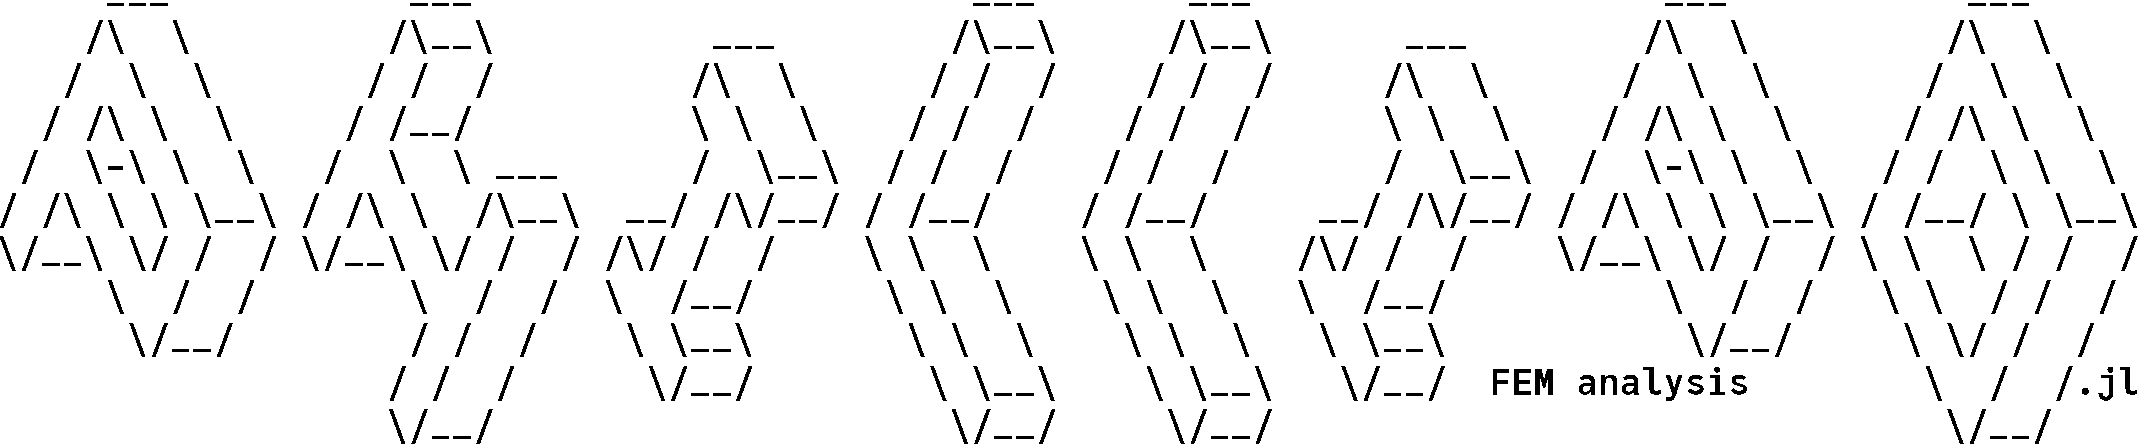
\includegraphics[width = \textwidth]{Figuras/logo_phillipo.pdf}
    \label{fig:log_phillipo}
\end{figure}

Neste capítulo é apresentado como é feita a distribuição e a instalação, e como se dá o funcionamento de PHILLIPO, dividido em duas partes. A primeira, descrevendo o fluxo de execução normal do programa, isto é, utilizando o GID como interface de pré e pós-processamento, e, a segunda, esmiuçando o código, tanto do módulo PHILLIPO, quanto dos arquivos de integração com o GID.

\section{Distribuição pelo Pkg.jl e importação dos \emph{Problems types} no GID}

O Pkg.jl é o gerenciador de pacotes anexado à Julia, tal como PIP é anexado ao Pyhton. Ele é responsável por distribuir, gerir e empacotar os módulos da linguagem, permitindo relacionar dependências e controlar versionamento. PHILLIPO é distribuído por meio do Pkg.jl, porém, não pelo repositório oficial\footnote{Há uma série de critérios para que um módulo seja adicionado ao repositório oficial do Pkg.jl, além disso, não é objetivo de PHILLIPO ser distribuido massivamente.}, mas pelo próprio repositório deste trabalho, que pode ser utilizado para o mesmo fim, pela função \emph{add}. A utilização do \emph{Pkg.jl} determinou a estrutura de a estrutura dos arquivos de código-fonte de PHILLIPO, conforme o próprio manual do pacote\footnote{Acessível em \url{https://pkgdocs.julialang.org/v1/}}.

Como PHILLIPO foi encapsulado em um módulo, pode ser facilmente distribuído iniciando uma sessão Julia e executando:
\begin{lstlisting}
    add https://github.com/lucas-bublitz/PHILLIPO.jl
\end{lstlisting}

O Pkg.jl então trata de buscar as dependências do módulo, isto é, os módulos que são importados para uso interno de PHILLIPO: o \emph{SparseArrays}, que fornece as estruturas e funções para alocar e manipular eficientemente matrizes esparsas, o \emph{LinearAlgebra}, implementação do LAPACK em Julia, e o \emph{JSON}, um parser de objetos em JSON para dicionários. No arquivo \emph{Projecy.toml} é possível encontrar tanto essa lista de dependência, e no \emph{Manifest.toml}, são listadas as dependências das dependências, isto é, quais módulos cada módulo importado por PHILLIPO importa para si. \footnote{O versionamento é importante pois permite que a compilação do pacote seja feita utilizando exatamente os códigos dos módulos de quando foi desenvolvido, assim baixando o risco de resultados inesperados devido a uma alteração no funcionamento de um módulo exterior ao que se trabalha. }

PHILLIPO utiliza a interface GID para gerar as malhas e definir as condições de contorno. A integração desses programas é feita pelo conjunto de arquivos presente presentes na pasta \emph{\textbackslash GID connections}: \emph{PHILLIPO.gid} e \emph{PHILLIPO3D.gid}, que são os \emph{Problem types} do GID para PHILLIPO, e \emph{link.jl}, que é o arquivo que é chamado pelo \emph{script} de execução do GID, e que importa o módulo PHILLIPO.jl e o executa. O conteúdo dessa pasta deve ser copiado para a pasta \emph{\dots\textbackslash GiD 16.1.6d \textbackslash ProblemTypes}, localizada onde o próprio GID está instalado\footnote{O caminho para a pasta \emph{ProblemTypes} pode variar de acordo com a versão do GID, e com o sistema operacional.}, para que sejam automaticamente carregados durante a inicialização do GID\footnote{Também é possível importar \emph{Problem types} dentro da interface do GID, entretanto, desse modo, a importação não é permanente.}.

\section{Fluxo de execução}

O fluxo de execução é uma ferramenta de projeto que tem como objetivo descrever a ordem e as condições que determinadas seções do código são executadas. A utilização de PHILLIPO.jl segue os digramas das figuras \ref{fig:fluxograma_GID} e \ref{fig:fluxograma_PHILLIPO}. Esses diagramas não representações simplificados e parciais, e não utilizam um padrão ou simbologia formal que é própria desses diagramas.
\begin{figure}[hbtp]
    \centering
    \caption{Fluxograma de execução: GID}
    \includegraphics[width = \textwidth]{Figuras/fluxograma_GID.pdf}
    \label{fig:fluxograma_GID}
\end{figure}

\begin{figure}[hbtp]
    \centering
    \caption{Fluxograma de execução: PHILLIPO.jl}
    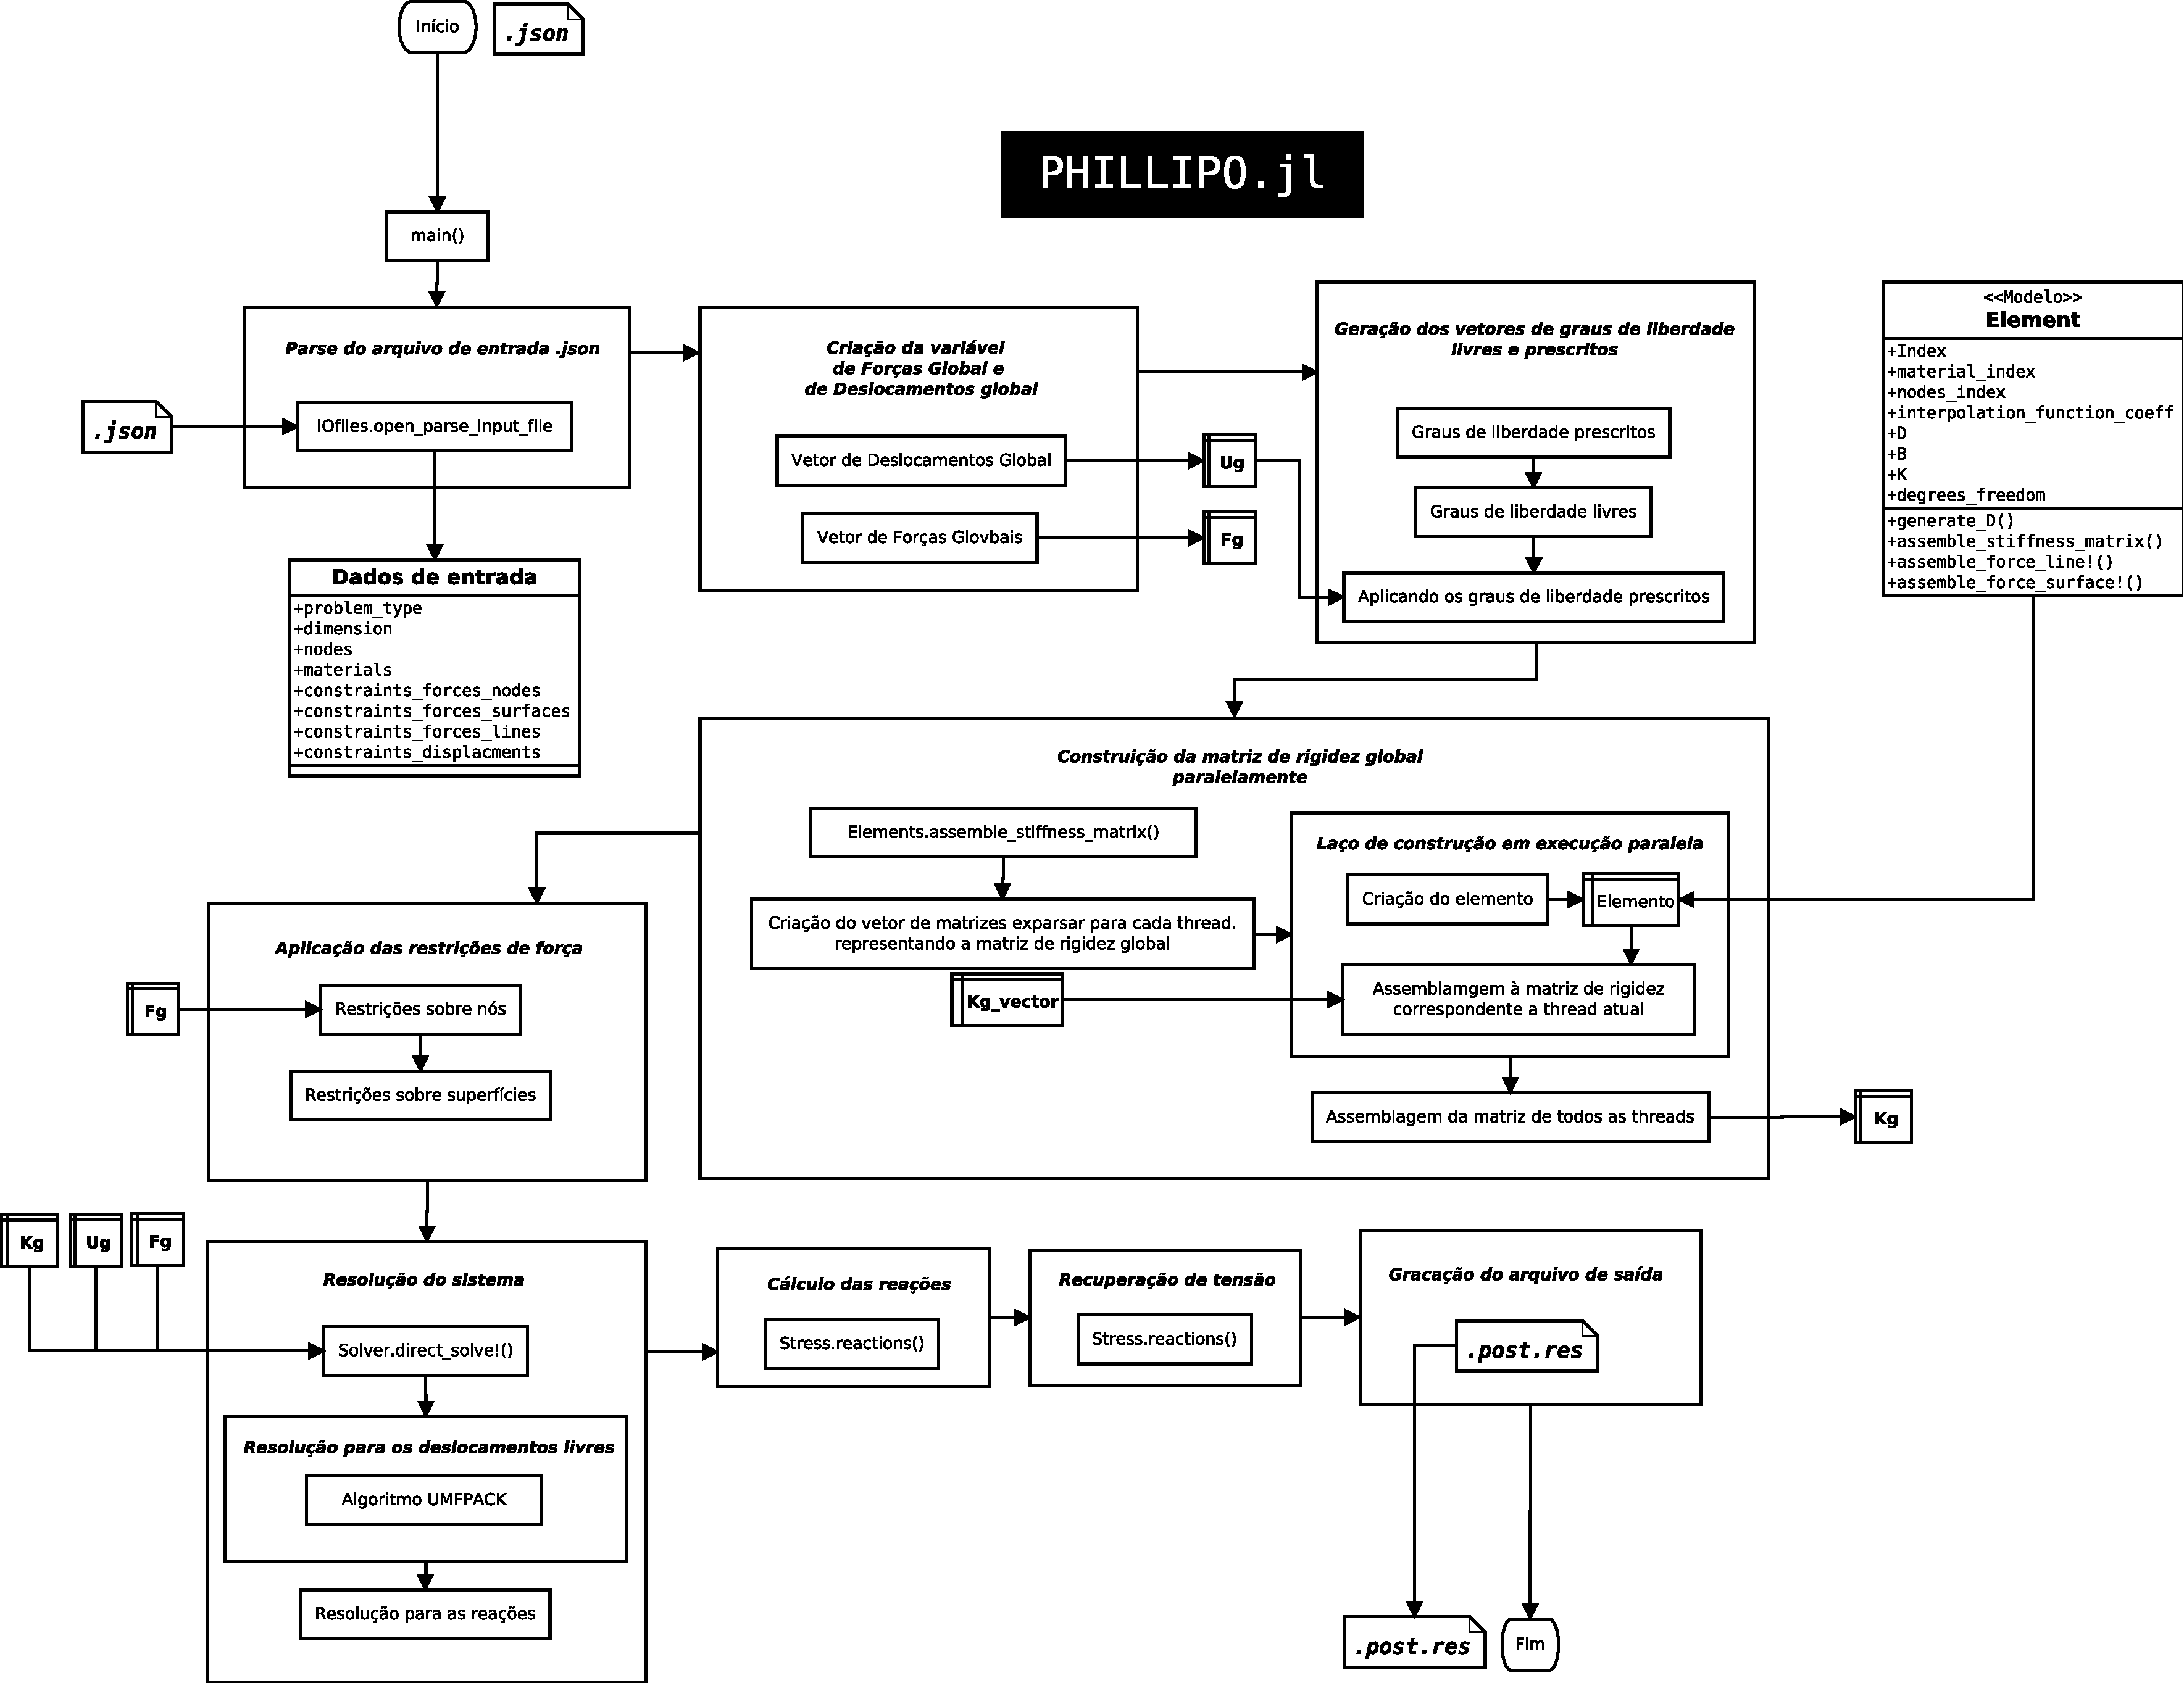
\includegraphics[width = \textwidth]{Figuras/fluxograma_PHILLIPO.pdf}
    \label{fig:fluxograma_PHILLIPO}
\end{figure}

Nesses diagramas, é possível separar a execução de uma utilização normal do software em três partes principais:

\begin{enumerate}
    \item Pré-processamento;
        Parte em que ocorre a criação da geometria, a definição das propriedades dos materiais, das condições de contorno e das cargas aplicadas, assim como a geração da malha e elementos.
    \item Processamento;
        Parte em que é chamada uma sessão Julia para carregar o módulo PHILLIPO.jl, que é responsável por ler os arquivos de entrada, e executar o algoritmo de elementos finitos, gerando os arquivos de saída para o GID.
    \item Pós-processamento;
        Parte em que o GID lê os arquivos de saída, e gera os gráficos de resultados.
\end{enumerate}

\subsection{Pré-processamento}

O pré-processamento é realizado totalmente pelo GID (figura \ref{fig:fluxograma_GID}), e consisti na definição da geometria, das condições de contorno, do material e na geração de malha, e segue:

\begin{enumerate}
    \item Definição do \emph{Problem type}. Caso o problema físico seja modelado em duas dimensões, deve-se escolher o \emph{Problem type} \emph{PHILLIPO}, caso seja modelado em três dimensões, deve-se escolher o \emph{Problem type} \emph{PHILLIPO3D}. Essa escolha define quais arquivos serão utilizados para a definição das condições de contorno, dos materiais, e como será a geração da malha. O GID cria então uma pasta onde os arquivos do problema serão salvos.

    \item \textbf{Definição da geometria do problema,} que pode ser tanto construída utilizando as ferramente CAE do próprio GID, como também, importada de um arquivo externo de algum outro software CAD cujo formato seja reconhecido pelo GID \footnote{O GID reconhece uma grande variedade de arquivo de entrada (sejam de geometria, malhas, condições de contorno), inclusive arquivos próprios de programas comerciais, como ANSYS e Abaqus;}.

    \item \textbf{Definição das características do material,} como também as condições de contorno: sejam elas deslocamentos sobre pontos, linhas e superfícies, ou carregamentos concentrados sobre pontos, ou carregamentos distribuídos sobre linhas e superfícies. \footnote{Carregamentos sobre linha só estão disponíveis para o \emph{Problem type} \emph{PHILLIPO}.}

    \item \textbf{Geração da malha,} que pode ser amplamente configuras pelas ferramentas oferecidas pelo GID para gerar malhas estruturadas ou não estruturas, com refinamentos em determinadas regiões, e com a possibilidade de se definir o tipo de elemento a ser utilizado. 
    \item \textbf{Chamamento da função de CALCULAR.}
\end{enumerate}

A função de CALCULAR do GID, executa o arquivo \emph{.bat} do \emph{problem type}: deleta possíveis arquivos de saída anteriores, e gera os arquivos de saída \emph{.dat}\footnote{Embora o arquivo esteja nomeado no formato \emph{dat} ele, na verdade, é um \emph{.json}, pois esse é o padrão de entrada para PHILLIPO.}, assim como os arquivos de \emph{log}, e cria a sessão Julia, chamando para ser executado nela o arquivo \emph{link.jl}. 

Na sessão Julia, o módulo PHILLIPO.jl é importado, momento em que ocorre a pré-compilação do código, e, em seguida, o chamamento da função principal do módulo \emph{PHILLIPO.main}, passando como parâmetros os caminhos para o arquivo \emph{.json} e o caminho de saída do resultado da análise, assim iniciando o processamento.

\subsection{Processamento}

O processamento é realizado dentro da sessão Julia, executando a função principal de \emph{PHILLIPO.main} (figura \ref{fig:fluxograma_PHILLIPO}), e consiste nas seguintes etapas:
\begin{enumerate}
    \item \textbf{Leitura do arquivo de entrada.} O arquivo \emph{.json} é lido e convertido em um dicionário pelo \emph{parser} JSON, cujos dados são distribuídos nas variáveis do problema.
    \item \textbf{Definição dos graus de liberdade livres e prescritos.} Conforme sãos as restrições de deslocamento, o programa calcula a numeração dos graus de liberdade prescritos, e os armazena em um vetor.
    \item \textbf{Construção da matriz global de rigidez paralelamente.} Nessa etapa, o programa chama as funções de construção de elemento paralelamente, utilizando uma macro do módulo \emph{Threads}, para construir a matriz global de rigidez, que é salva no formato COO (um formato de matriz esparsa que armazena os valores em um vetor único cuja ordem não importa para a interpretação da matriz, o que facilita a execução paralela). Após a construção da matriz global de rigidez, é feita a conversão para o formato de matriz esparsa CSR. 
    \item \textbf{Aplicação das restrições de forças.} As restrições de forças são aplicadas sobre o vetor de forças prescritas. Dependendo do tipo (sobre linhas ou superfícies), são calculadas as forças nodais equivalentes.
    \item \textbf{Resolução do sistema.} Com a matriz global de rigidez e o vetores de deslocamentos e forças nodais, o programa decompõe o sistema pelos graus de liberdade livres e prescritos, e o resolve diretamente, utilizando o método mais apropriado, determinado pelo módulo \emph{LinearAlgebra}, levando em consideração as características da matriz de rigidez global.
    \item \textbf{Cálculo das reações e recuperação de tensão.} O programa calcula as reações de apoio, utilizando os graus de liberdade prescritos, e, em seguida, calcula as tensões, chamando, novamente, as funções de construção de elementos para resgatar as matrizes de rigidez locais.
    \item \textbf{Geração do arquivo de saída.} O programa gera o arquivo de saída, no formato \emph{.dat}, que é lido pelo GID para gerar os gráficos de resultados.

\end{enumerate}

Com o fim da execução da função principal, é encerrada a sessão Julia e, e é chamado o programa Notepad para a abrir o arquivo \emph{.log}, onde algumas informações de debug foram impressas durante o processamento. 

\subsection{Pós-processamento}


O Pós-processamento é realizado pelo GID, e consiste num conjunto de ferramentas de plotagem, com diversas formas de visualizar todo os dados impressos no arquivo de saída.

\section{Integração com GID}

O GID é um software utilizado como pré e pós-processamento (ver figuras \ref{fig:gid_1} e \ref{fig:gid_2}). Com ele é possível criar a geometria do problema, definir as propriedades dos materiais, as condições de contorno, as cargas aplicadas, e, principalmente, gerar a malha de elementos. Além de se ser possível a integração com um \emph{solver} qualquer, por meio de um conjunto de arquivos de entrada e saída (ambos configurados de forma a permitir uma certa flexibilidade nessa integração), cuja execução é controlada por um \emph{script} em Batch, o que possibilita a automatização do processo de simulação. Nesta seção é abordado como é feita e integração entre o GID e PHILLIPO, por meio das pastas \emph{PHILLIPO.gid} e \emph{PHILLIPO3D.gid}, sendo que, como a nomeação dos arquivos sugere, a primeira é utilizada para problemas bidimensionais, e a segunda para problemas tridimensionais.

\begin{figure}[hbtp]
    \centering
    \caption{Exemplo de pré-processamento de geometria no GID}
    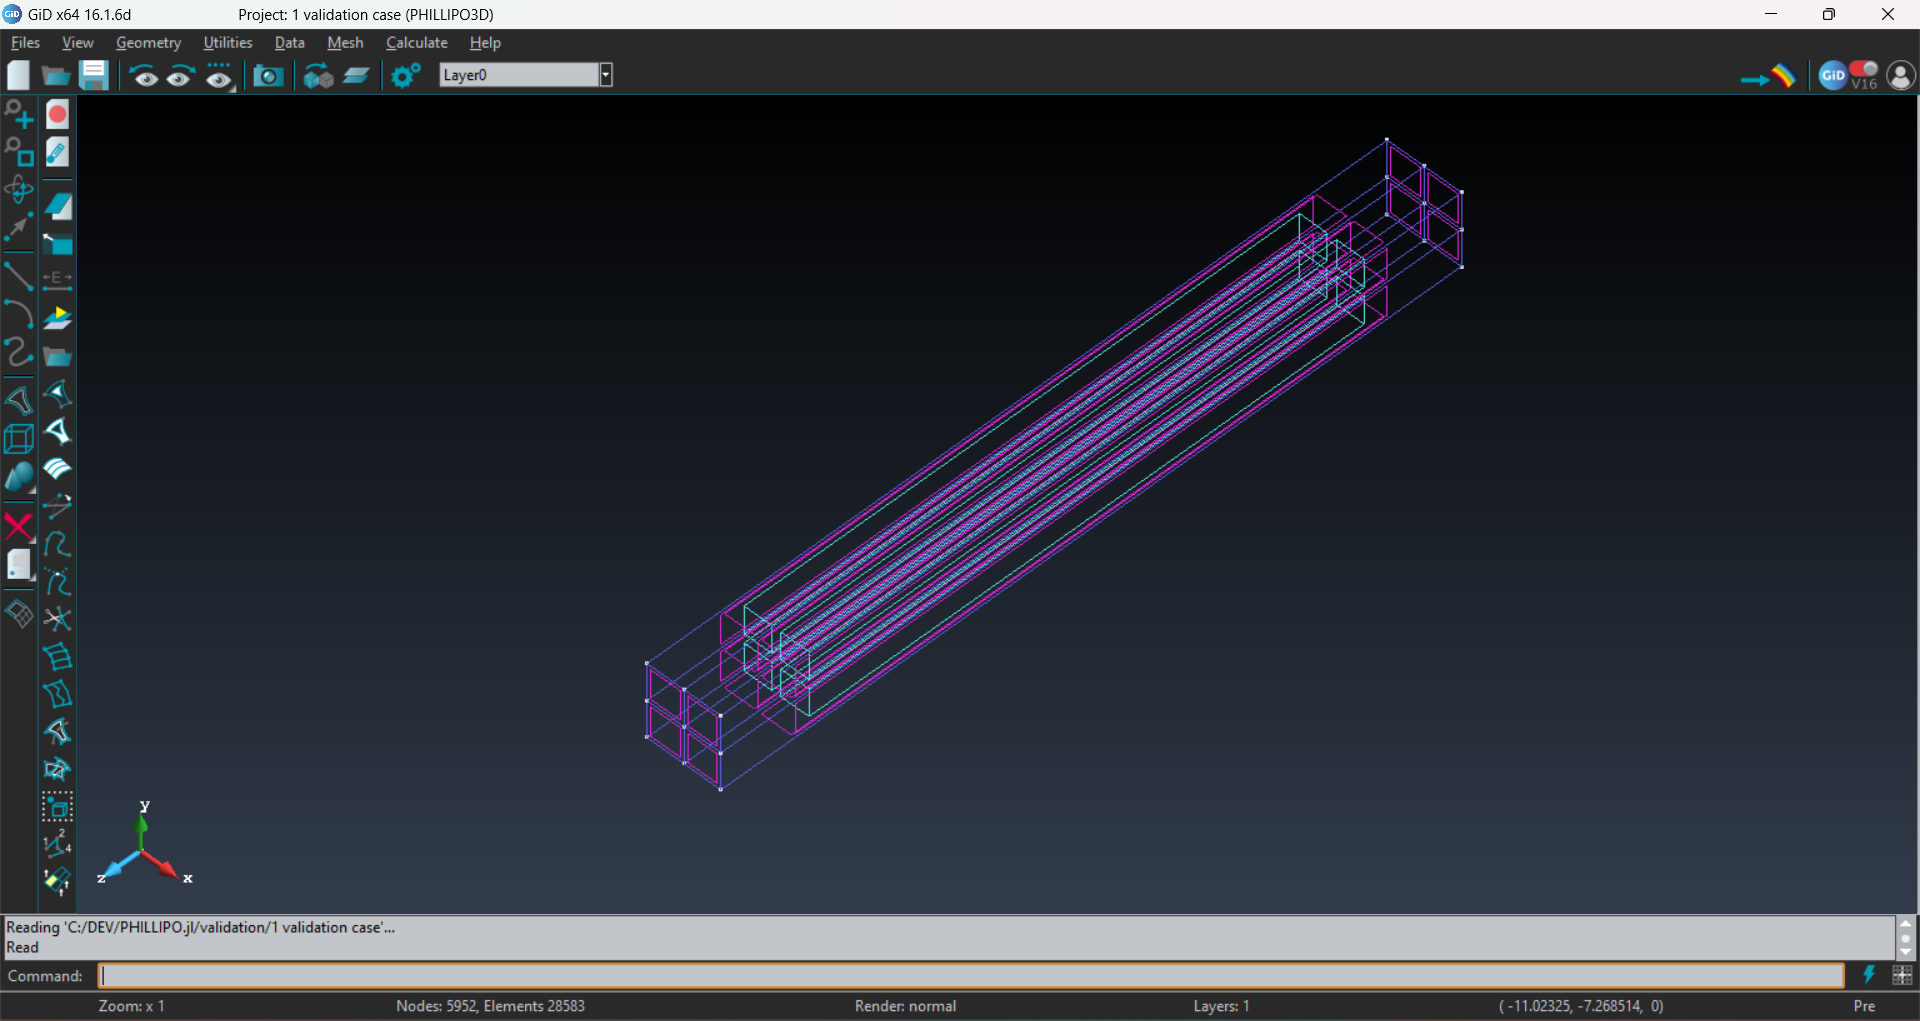
\includegraphics[width = \textwidth]{Figuras/gid_1.png}
    \label{fig:gid_1}
\end{figure}

\begin{figure}[hbtp]
    \centering
    \caption{Exemplo de pós-processamento no GID}
    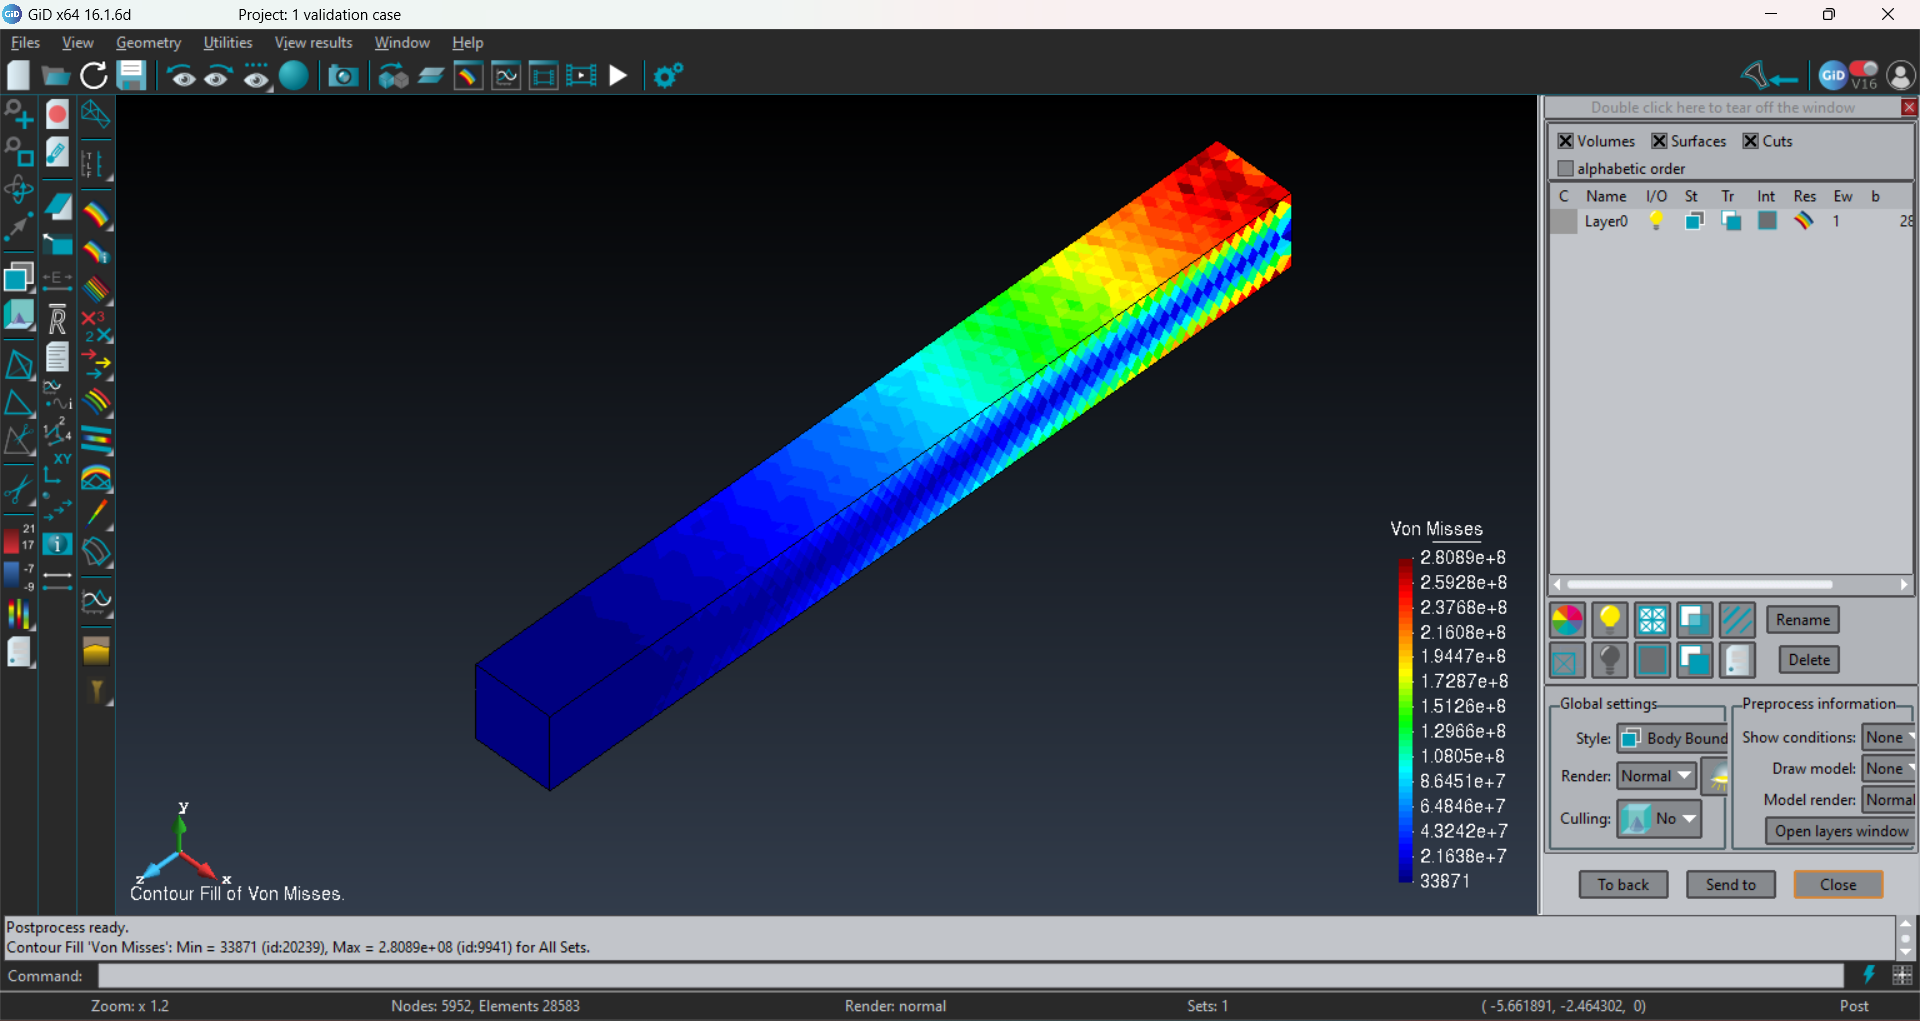
\includegraphics[width = \textwidth]{Figuras/gid_2.png}
    \label{fig:gid_2}
\end{figure}


\subsection{PHILLIPO.gid}

O GID pode ser configurado para operar como pré e pós-processamentos de diversos programas, como o Abaqus, o Ansys, o Calculix..., por meio de um \emph{Problem type}, que é como o GID chama o conjunto de arquivos que configuram o formato de saída dos dados, a criação de determinadas propriedades para as condições de contorno e materiais, como também automatizar a execução da simulação, chamando o programa. Pode-se dizer que o \emph{Problem type} é uma interface para que as informações contidas nos arquivos gerados pelo GID (geometria, malha, condições de contorno etc.) sejam salvas em um formato que o programa, o \emph{solver}, possa interpretar, ao passo que o \emph{script} de execução automatiza o chamamento desse, e a simulação seja iniciada. 

Na pasta \emph{PHILLIPO.gid} é possível encontrar os seguinte arquivos:

\begin{enumerate}
    \item \emph{PHILLIPO.cnd}: define as condições de contorno e como são aplicadas;
    \item \emph{PHILLIPO.prb}: define as entradas de informações gerais;
    \item \emph{PHILLIPO.mat}: define as características dos materiais utilizados para os elementos;
    \item \emph{PHILLIPO.bas}: configura o arquivo de saída do GID para ser interpretado por PHILLIPO.jl;
    \item \emph{PHILLIPO.bat}: \emph{script} para chamar uma sessão Julia, chamando \emph{link.jl};
    \item \emph{link.jl}: importa o módulo PHILLIPO e o executa.
\end{enumerate}

O primeiro arquivo do \emph{Problem type} de PHILLIPO é \emph{PHILLIPO.cnd}, que define as condições de contorno e sobre quais entidades, leia-se nós, elementos ou geometrias (superfícies, volumes, linhas etc.), são aplicadas, por meio de uma sintaxe específica \footnote{No manual do usuário do GID, acessível em \url{https://gidsimulation.atlassian.net/wiki/spaces/GUM/overview}, é possível encontrar a descrição o funcionamento de toda essa sintaxe, que compreende desde esse arquivo de condições de contorno, como também, dos outros que compões a construção do \emph{problem type}.}, uma forma de marcação de texto, que é interpretada pelo GID.

\begin{figure}[hbtp]
    \caption{Parte do arquivo de condições de contorno: PHILLIPO.cnd}
    \lstinputlisting[lastline=10]{../GID connection/PHILLIPO.gid/PHILLIPO.cnd}
    \label{fig:PHILLIPO.cnd}
\end{figure}

Em sua representação parcial, da figura \ref{fig:PHILLIPO.cnd}, é possível notar a construção de uma condição de contorno por meio de um bloco que inicia na linha 1, com a expressão \emph{CONDITION: Constraint\_displacement\_point}, que também nomeia esta condição, referente a restrição de deslocamento em pontos (entidade geométrica discretizada por um nó), e que acaba com \emph{END CONDITION}. Dentre essas linhas, são definidas as formas e os valores que essa condição vai aplicar sobre a geometria selecionada, neste caso, os pontos. Na linha 2, é definido, justamente, sobre qual entidade geométrica se aplica essa condição: pontos. Na próxima linha, é definido como que essa informação, que foi associada à entidade geométrica se traduz na malha: essa condição é aplicada sobre os nós que cujo ponto foi discretizado. \footnote{Isso se deve porque a malha é criada sobre a geometria, posteriormente à aplicação das condições de contorno sobre aquela.} As linhas seguintes, 4 a 9, se referem aos valores da condição, neste caso, aos deslocamentos prescritos sobre os nós nas direções de \emph{X}, \emph{Y} e \emph{Z}. 

Na condição \emph{Constraint\_force\_line} (figura \ref{fig:PHILLIPO.cnd_2}), o processo é análogo. A restrição de carregamento uniforme é aplicada sobre uma linha (o tipo de geometria), e, diferentemente da anterior, é traduzida sobre as faces. Nesse caso bidimensional, é o segmento de reta determinado pelos nós nas extremidades. Os campos \emph{X}, \emph{Y} e \emph{Z}, referem-se ao vetor dessa carregamento uniformeS.

\begin{figure}[hbtp]
    \caption{Parte do arquivo de condições de contorno: PHILLIPO.cnd}
    \lstinputlisting[firstline=36,lastline=45]{../GID connection/PHILLIPO.gid/PHILLIPO.cnd}
    \label{fig:PHILLIPO.cnd_2}
\end{figure}

O arquivo \emph{PHILLIPO.prb} (figura \ref{fig:PHILLIPO.prb}) define as entrada de informações gerais ao problema, ou seja, que não são aplicados diretamente sobre a geometria. Somente um campo foi utilizado e se refere ao tipo do estado plano (EPD ou EPT). A sintaxe da linha 3 é indica que esse campo só possa ser preenchido por essas duas opções, no formato \emph{drop-down list}.
\begin{figure}[hbtp]
    \caption{Arquivo de dados gerais: PHILLIPO.prb}
    \lstinputlisting[firstline=1,lastline=8]{../GID connection/PHILLIPO.gid/PHILLIPO.prb}
    \label{fig:PHILLIPO.prb}
\end{figure}

O arquivo \emph{PHILLIPO.mat} (figura \ref{fig:PHILLIPO.mat}) define as características dos materiais implementados. Somente um material foi definido, o aço AISI 4340, com os campos de módulo de elasticidade, coeficiente de Poisson e massa específica.

\begin{figure}[hbtp]
    \caption{Arquivo de materiais: PHILLIPO.mat}
    \lstinputlisting[firstline=1,lastline=8]{../GID connection/PHILLIPO.gid/PHILLIPO.mat}
    \label{fig:PHILLIPO.mat}
\end{figure}

O arquivo \emph{PHILLIPO.bas} configura o arquivo de saída do GID. Esse arquivo intercala o conteúdo explicito do arquivo de saída (as partes invariáveis), com trechos de programação, responsáveis por imprimir os valores dinâmicos, aqueles referentes ao problema em si, como as coordenadas dos nós, a conectividade dos elementos etc.\footnote{Esse modo de compor os arquivo, misturando textos estáticos e programação é similar aos arquivos em PHP. Isso numa utilização mais clássica.} A separação entre texto e programa se dá pelo caractere \emph{*} no início da linha, indicando que toda ela é uma instrução para ser executada. 

O arquivo gerado é do formato \emph{.json}, o que pode ser não usual para aplicações do MEF. Entretanto, esse formato é amplamente utilizado para troca de dados entre aplicações, e, por isso, pode ser facilmente lido por um módulo já consolidado em Julia, o \emph{JSON.jl}\footnote{JSON se refere a \emph{JavaScript Object Notation}, um formato de texto para representar objetos na linguagem JavaScript, que se tornou padrão na implementação de APIs.}. 

Para gerar as listas de elementos triangules, foi escrito o seguinte código, dentro do arquivo emph{PHILLIPO.bas}:
\lstinputlisting[firstline=10,lastline=16]{../GID connection/PHILLIPO.gid/PHILLIPO.bas}
Em cada linha, os nós são definidos por listas, cujos valores representam as componentes $x$ e $y$ respectivamente. A numeração dos nós é implícita pela ordem da lista de \emph{"nodes"}.

Na linha 1 é definido o nome do campo \emph{"nodes"}, separado pelo características \emph{:} inicia a declaração do valor daquele campo: uma lista \emph{[}\footnote{Essa sintaxe de listas e \emph{literals} é próprio do JavaScript.}. Na linha 2, é iniciado um laço de repetição, que percorre todos os nós, e, para cada um, é adicionado um elemento à lista, que é composto por um par de coordenadas, separadas por vírgula, e envolvidas por colchetes, pois cada nó é presentando por um vetor que contem suas coordenadas. Na linha 5, é fechado o laço de repetição, e, na linha 6, é fechado o campo \emph{]}. 

Esse padrão se repete para o elementos também, com a diferença que estes, dependendo do seu tipo (CST ou tetraedro), são listas dentro da tupla que representa dos os elementos. Na figura \ref{fig:PHILLIPO.bas}, é possível nota essa hierarquia dos dados na estrutura de entrada de PHILLIPO. O elementos são separados pela forma das funções de interpolação. Para o CST, as funções são linear, então esses elementos são gravados dentro da chave \emph{"linear"}. 

Vale ressaltar também como as condições de contorno são gravas. Como as restrições de deslocamento sempre são sobre nós, só a uma lista desse tipo. Já os carregamentos, para serem aplicados no MEF, precisam ser convertidos para forças nodais, e, para tanto, é necessário utilizar as funções de interpolação que dependem do elemento. Por conta disso, são gravadas as condições de contorno de carregamento sobre as entidades geométricas: linhas e superfícies, por meio dos nós, de forma que o PHILLIPO se encarrega de calcular, utilizando as funções de interpolação, as forças nodais equivalentes sobre o elemento que a contém. Na linha 35, da figura \ref{fig:PHILLIPO.bas}, uma restrição de força é descrita: a primeira posição se refere a numeração que o GID deu para aquela entidade de linha, os dois valores seguintes são os identificadores dos que definem a entidade, e os valores restantes são as componentes do carregamento.

\begin{figure}[hbtp]
    \caption{Arquivo de saída do quarto caso de verificação: 4 verification case.dat}
    \lstinputlisting{../verification/4 verification case/4 verification case.gid/4 verification case.dat}
    \label{fig:PHILLIPO.bas}
\end{figure}



O arquivo \emph{PHILLIPO.bat} (figura \ref{fig:PHILLIPO.bat}) é um \emph{script} que é chamado pela função CALCULAR do GID, para iniciar a análise do problema. É um arquivo de linhas de comando (ou arquivo de lote)\footnote{Comandos utilizados dentro do terminal do sistema: o CMD.} para o sistema operacional Windows\footnote{Por conta disso, o \emph{PHILLIPO.gid} só funciona em sistemas Windows.}.

Nas linhas 1 a 3, são feitas as exclusões de possíveis arquivos restantes de análises passadas. Na linha 4, é chamada a sessão Julia, passando como parâmetro o arquivo \emph{link.jl}, o caminho absoluto do arquivo de entrada \emph{.dat} e o local em que o arquivo de saída deve ser gravado. No final da linha, os operadores right-shift \emph{>>} redirecionam o debug da execução de PHILLIPO para o arquivos \emph{.log} e \emph{.error.log}. Na linha 5, o arquivo log de erro é aglutinado ao arquivo de log para que, quando a linha 5 for executada, o aplicativo Notepad exiba os dois conteúdos juntos\footnote{Assim foi implementado porque se o mesmo arquivo receber o fluxo de texto, o conteúdo dos erros sobrescrevem aos normais}. 

A flag \emph{-t} com o parâmetro \emph{auto} na linha 4, indica que a sessão Julia deve ser iniciado utilizado um número de threads disponibilizados pelo sistema \footnote{O parâmetro pode ser alterado para forçar a sessão Júlia a usar mais threads.}. Isso é importante para que ocorra a montagem da matriz global de rigidez paralelamente.

\begin{figure}[hbtp]
    \caption{Arquivo de execução: PHILLIPO.bat}
    \lstinputlisting{../GID connection/PHILLIPO.gid/PHILLIPO.bat}
    \label{fig:PHILLIPO.bat}
\end{figure}

O arquivo \emph{link.jl} (figura \ref{fig:link.jl}) é o arquivo que executado dentro da sessão Julia. Ele recebe esse nome porque é o arquivo que faz a ligação entre a execução do GID e o módulo PHILLIPO.jl, e, por não estar previsto dentro da estrutura de um \emph{problem type}, recebe um nome diferenciado. Nele é apenas importado o módulo PHILLIPO.jl  (linha 1) e chamado a função principal do módulo (linha 2), passando como parâmetros o caminho para o arquivo de entrada e o caminho para a gravação do arquivo de saída \footnote{ARGS é um vetor presente em toda a sessão Julia, que recebe os parâmetros passados para o executável que a iniciou.}. A última linha é responsável por garantir o encerramento da sessão Julia.

A macro \emph{@time} é responsável por fornecer algumas informações sobre o tempo de execuções do módulo (como também memória alocada e tempo dedicado à compilação ao \emph{Garbage Collector}). É uma ferramenta de debug, e seu retorno é impresso no arquivo \emph{.log}.

\begin{figure}[hbtp]
    \caption{Arquivo de execução: link.jl}
    \lstinputlisting{../GID connection/PHILLIPO.gid/link.jl}
    \label{fig:link.jl}
\end{figure}

\section{Estrutura do módulo PHILLIPO.jl}

O código-fonte de PHILLIPO foi organizado em seis módulos, ao longo de sete arquivos \emph{.jl}, agrupando as funções em categorias conforme sua aplicação. O início da definição do módulo de PHILLIPO é o arquivo homônimo, localizado na raiz da pasta \emph{src} do repositório. São os arquivos:

\begin{enumerate}
    \item \textbf{\emph{PHILLIPO.jl}}: define o módulo PHILLIPO e a função principal;
    \item \textbf{\emph{includes.jl}}: juntas as importações dos módulos internos;
    \item \textbf{\emph{IOfiles.jl}}: módulo interno que define as funções de leitura e escrita de arquivos;
    \item \textbf{\emph{Elements.jl}}: módulo interno que  define as estruturas dos elementos e suas funções;
    \item \textbf{\emph{Matrices.jl}}: módulo interno que define a estrutura das matrizes COO;
    \item \textbf{\emph{Solver.jl}}: módulo interno que executa a resolução do sistema;
    \item \textbf{\emph{Stress.jl}}: módulo de recuperação de tensões.
\end{enumerate}


\subsection{PHILLIPO.jl}

O arquivo \emph{PHILLIPO.jl} é o que define o próprio módulo, e por contada disso é homônimo. Nele é se encontra a função principal \emph{main}, que vai conduzir toda a parte do processamento da análise \footnote{Pode-se pensar na função principal como um ponto de partida do software, um \emph{int main()} como em C.}. Na figura \ref{fig:phillipo.jl}, uma parte desse arquivo é reproduzida. 

\begin{figure}[hbtp]
    \caption{Parte do arquivo principal do módulo: PHILLIPO.jl}
    \lstinputlisting[firstline = 14, lastline = 32, language=python]{../src/PHILLIPO.jl}
    \label{fig:phillipo.jl}
\end{figure}

A primeira linha é a declaração da abertura do módulo, cujo nome é precedido pela keyword \emph{module}. As linhas 3 a 10 são responsáveis por importar os módulos utilizadas. Nessa parte é importante salientar o seguinte: os módulos internos, aqueles definidos como bibliotecas explícitas dentro de PHILLIPO são incluídos aninhadamente pela inclusão do arquivo \emph{includes.jl}, e para serem chamados à pré-compilação devem ser importados diretamente, conforme as linhas 9 a 13\footnote{Os nomes do módulos internos devem ser seguidos de um ponto quando forem importados. Isso é devido a localização dos arquivos do sistema de Julia. Sem essa notação, a sessão Julia vai tentar buscar nos módulos instaladas na aquele ambiente, e não os declarados explicitamente no código.}. As Inclusões são a forma de se particionar os arquivos do módulo, fazendo com que sejam aglutinados naquela linha em que são chamados. Para o \emph{Pkg.jl}, todo o código se torna apenas um arquivo contínuo.

Na linha 16, a função \emph{main} é definida, e recebe dos valores: o caminho para o arquivo \emph{.dat} de dados de entrada, o caminho para o arquivo de saída. Após essas linha, o chamamento das funções segue o descrito no fluxo de execução do processamento, na subseção anterior. Vale ressaltar que nessa função estão presentes uma série de impressões, \emph{prints}. Esses são os \emph{debugs} já mencionados, que vão compor o arquivo \emph{.log}\footnote{Existem outros modos de realizar o debug, utilizando a macro \emph{@debug}.}.

A parte posterior da função principal é a leitura dos dados de entrada, chamando a função \emph{IOfiles.open\_parse\_input\_file}, na linha 5 da figura \ref{fig:phillipo.jl_2}, retornando um dicionário na variável \emph{input\_dict}, cujos dados, nas linhas seguintes, são distribuídos às variáveis principais do problema:

\begin{enumerate}
    \item \textbf{\emph{problem\_type}}: referente ao tipo do problema (EPT, EPD ou tridimensional);
    \item \textbf{\emph{nodes}}: vetor de vetores das coordenadas dos nós ordenados;
    \item \textbf{\emph{materials}}: vetor de materiais declarados;
    \item \textbf{\emph{constraints\_forces\_nodes}}: vetor dos vetores de restrições de força sobre nós;
    \item \textbf{\emph{constraints\_forces\_lines}}: vetor dos vetores de restrições de força sobre linhas;
    \item \textbf{\emph{constraints\_forces\_surfaces}}: vetor dos vetores de restrições de força sobre superfícies;
    \item \textbf{\emph{constraints\_forces\_displacements }}: vetor dos vetores de restrições de deslocamento sobre nós.
\end{enumerate}

Também são definidas, com espaço previamente alocado, os vetores deslocamento nodais global e forças nodais globais, respectivamente \emph{Ug} e \emph{Fg} (linhas 36 e 37). As linhas de chamando a função \emph{pop!} servem para retirar os valores \emph{null} dos fins dos vetores\footnote{Isso se dá pela forma como a programação no arquivo \emph{.bas} foi realizada. Nos arquivos \emph{.json} não são permitidos os \emph{Trailing commas}, e, para contornar essa situação, em cada loop foi adicionado um valor \emph{null} que é retirado justamente nesta parte do programa.}.

\begin{figure}[hbtp]
    \caption{Parte do arquivo principal do módulo: PHILLIPO.jl}
    \lstinputlisting[firstline = 29, lastline = 65, language=python]{../src/PHILLIPO.jl}
    \label{fig:phillipo.jl_2}
\end{figure}

A próxima parte do arquivo cria os vetores de graus de liberdade prescritos e livres, respectivamente \emph{dof\_prescribe} e \emph{dof\_free}, e, em seguida, já aplicada as restrições de deslocamentos nodais sobre os graus respectivos no vetor \emph{Ug}, como está na figura \ref{fig:phillipo.jl_3}.

Os graus de liberdade são numerados de acordo com a numeração dos nós sequencialmente, de modo que o nó de número $1$ tenha os graus $1$, $2$ e $3$, e um certo nó $n$, tenha os graus $3n-2$, $3n-1$ e $3n$, para um problema tridimensional. Para o caso bidimensional, a regra é similar: o nó $n$ tem o graus $2n-1$ e $2n$. Essas regras estão implementadas na forma de funções anônimas (linhas 4 e 12). 

A função \emph{map} mapeia cada elemento do vetor de restrições de deslocamento para um vetor de graus de liberdade restritos. Para unir esses vetores, a função \emph{reduce} aplica uma função binária, no caso a função \emph{vcat}, entre os elementos do vetor, e retorna um único vetor com todos os graus de liberdade \footnote{Essa forma de construir essa parte do código é um exemplo de um aspecto de programação funcional.}. 

\begin{figure}[hbtp]
    \caption{Parte do arquivo principal do módulo: PHILLIPO.jl}
    \lstinputlisting[firstline = 67, lastline = 84, language=python]{../src/PHILLIPO.jl}
    \label{fig:phillipo.jl_3}
\end{figure}

A próxima parte do arquivo, figura \ref{fig:phillipo.jl_4}, é o chamamento da função da montagem da matriz de rigidez global \emph{Elements.assemble\_stiffness\_matrix}, que a retorna no formato CSR para a variável \emph{Kg}. 

\begin{figure}[hbtp]
    \caption{Parte do arquivo principal do módulo: PHILLIPO.jl}
    \lstinputlisting[firstline = 87, lastline = 89, language=python]{../src/PHILLIPO.jl}
    \label{fig:phillipo.jl_4}
\end{figure}

Em seguida, a função principal aplica as restrições de força(figura \ref{fig:phillipo.jl_5}) de dois modos: diretamente sobre o vetor de forças nodais globais, e, chamando as funções que calculam as forças nodais equivalentes, para os casos de carregamentos sobre linhas e superfícies.

Na aplicação de forças nodais prescritas, é primeiro calculado os graus de liberdade as forças serão aplicadas, num procedimento idêntico ao realizado para as restrições de deslocamento. Em seguida, o vetor \emph{Fg} é acessado sobre essas posições dos graus de liberdade para receber todas as forças prescritas na forma de um vetor único, por uma concatenação de vertical de vetores.

As outras formas de restrições de força são aplicadas por meio das funções \emph{Elements.assemble\_force\_surface!} e \emph{Elements.assemble\_force\_line!}.

\begin{figure}[hbtp]
    \caption{Parte do arquivo principal do módulo: PHILLIPO.jl}
    \lstinputlisting[firstline = 92, lastline = 112, language=python]{../src/PHILLIPO.jl}
    \label{fig:phillipo.jl_5}
\end{figure}

A próxima parte do arquivo, figura \ref{fig:phillipo.jl_6}, é a resolução do sistema, chamando a função \emph{Solver.direct\_solve!}. Como essa função recebe os vetores de deslocamentos e forças nodais globais, não retorna nada, pois já aplicada a resolução do sistema sobre esses vetores. Em seguida, ocorre o cálculo das reações pela função \emph{Stress.reactions}, que retorna o vetor de reações \emph{R} e seu somatórios \emph{Re\_sum}, cujo propósito é verificar se o resultado do sistema está em equilíbrio.

O cálculo das tensões é feito pela função \emph{Stress.recovery}, para as variáveis \emph{\sigma} e \emph{\sigma vm}, respectivamente, o vetor de tensões na notação de Voigt e o vetor de tensões de von Mises.

\begin{figure}[hbtp]
    \caption{Parte do arquivo principal do módulo: PHILLIPO.jl}
    \lstinputlisting[firstline = 115, lastline = 125, language=python]{../src/PHILLIPO.jl}
    \label{fig:phillipo.jl_6}
\end{figure}

A última parte do arquivo \emph{PHILLIPO.jl} é a escrita do próprio arquivo de saída \emph{.dat}, por meio do módulo interno \emph{IOfiles}. Nessa etapa é preciso inserir uma série de cabeçalhos no arquivo para que o GID possa interpretá-los corretamente. 

Finalizada a escrita sobre o arquivo de saída, a função principal é encerrada.

\subsection{Elements.jl e paralelismo na montagem da matriz de rigidez global}

O módulo \emph{Elements.jl} é divido em duas seções: a definição dos \emph{structs} do tipos de elementos, compostos pelos dados necessários para montar a matriz de rigidez local e uma função de criação, e as funções relativas à montagem da matriz de rigidez e da aplicação dos carregamentos sobre o sistema.


O elemento CST, por exemplo, é definido pelo \emph{struct} \emph{TriangleLinear}, e contém os seguintes dados na forma de variáveis:

\begin{enumerate}
    \item \textbf{\emph{nodes}}: vetor de vetores das coordenadas dos nós ordenados;
   \item \textbf{\emph{index}}: número de identificação do elemento;
   \item \textbf{\emph{material\_index}}: número de identificação do material;
   \item \textbf{\emph{nodes\_index}}: conectividade;
   \item \textbf{\emph{interpolation\_function\_coeff}}: coeficientes das funções de interpolação na forma da matriz $\bm{X}^{-1}$, equação \ref{eq:matriz_x};
   \item \textbf{\emph{D}}: matriz constitutiva do material $\bm{C}$;
   \item \textbf{\emph{B}}: matriz deformação-deslocamento $B$, equação \ref{eq:deformacao_deslocamento};
   \item \textbf{\emph{K}}: matriz de rigidez local;
   \item \textbf{\emph{degrees\_freedom}}: graus de liberdade do elemento;
\end{enumerate}

A função homônima \emph{TriangleLinear} é responsável por construir o elemento CST, conforme as relações estabelecidas no capitulo de Elementos Finitos. Ela é uma abstração superior da função \emph{new}, que de fato vai preencher as variáveis listadas acima e retornar o próprio \emph{struc} do elemento específico.

Primeiramente, a função de construção do CST remaneja os dados de entrada para as variáveis do \emph{Struc}: \emph{index}, \emph{material\_index} e \emph{nodes\_index}, e preenche os as variáveis $i$, $j$ e $m$ os vetores de coordenadas dos respectivos nós, para, em seguida, construir a matriz $\bm{X}$ na variável \emph{position\_nodes\_matrix}. Em seguida, calcula a matriz $\bm{X}^{-1}$, e a área do elemento, variável \emph{\Delta}. A matriz $B$ é calculada com os os temos da inversa matriz $\bm{X}^{-1}$, cujas colunas foram distribuídas nas variáveis \emph{a}, \emph{b} e \emph{c}, que representam os termos $\alpha$, $\beta$ e $\gamma$ da equação \ref{eq:matriz_x}. 

Por fim, a função de construção calcula a matriz de rigidez local, \emph{K}(pela fórmula da equação \ref{eq:matriz_local}), determina os graus de liberdade do nós que compõe o elemento, na vetor \emph{degrees\_freedom}, e, por meio da função \emph{new}, retorna o elemento.

\begin{figure}[hbtp]
    \caption{\emph{Struct} do elemento CST: TriangleLinear}
    \lstinputlisting[firstline = 25, lastline=71, language=python]{../src/modules/Elements.jl}
    \label{fig:TriangleLinear}
\end{figure}

A função \emph{assemble\_stiffness\_matrix}, figura \ref{fig:asm}, é responsável pela montagem da matriz de rigidez global paralelamente, utilizando a estrutura de dados COO, para separar o processo em \emph{threads} diferentes.    

\begin{figure}[hbtp!]
    \caption{Função assemble\_stiffness\_matrix do arquivo: Elements.jl}
    \lstinputlisting[firstline = 170, lastline=208]{../src/modules/Elements.jl}
    \label{fig:asm}
\end{figure}


Primeiramente, na linha 6, é criada a variável \emph{Kg\_vector}, um vetor de tamanho equivalente ao número de \emph{threads} disponibilizadas pela sessão Julia, cujas posições são matrizes no formato COO, que representam a matriz de rigidez global.

A macro \emph{Threads.@threads} transforma a execução do loop na linha 12, sobre todos os elementos de síncrona para assíncrona, de modo que as iterações sejam distribuídas, em tempo de execução, pelas \emph{Treads}, ou seja, as iterações são armazenadas na forma de uma fila, um \emph{pipe}, e conforme as \emph{Threads} vão ficando disponíveis, elas vão retirando as iterações da fila e as executando.

Dentro do loop, o elemento respectivo é criado pela sua função construção do \emph{strucs}. A função \emph{Matrices.add!}, então, soma a matriz local desse elemento, sobre os seus graus de liberdade, na matriz global referente a posição do vetor \emph{Kg\_vector} correspondente a \emph{Thread} em que a iteração está sendo executada.

A função \emph{Matrices.add!} não soma de fato os valores, apenas concatena os novos nos vetores que compõe o formato COO implementado. A soma de fato é realizada pela função \emph{Matrices.sum} depois de ser encerrado o loop.

Os \emph{threads} são marcados por identificadores numéricos, que podem ser acessados pela função \emph{Threads.threadid}. O chamamentos dessa função dentro do loop garante que a soma da matriz local se dê sobre uma posição do vetor \emph{Kg\_vector} por vez.

Caso não fosse realizado essa divisão de variáveis para a execução assíncrona, as iterações poderiam acessar a mesma posição ao mesmo tempo. Quando isso ocorre, uma iteração é descartada pela sessão, fazendo com que a matriz de rigidez seja montada errada.

Finalizado o loop, as matrizes do vetor \emph{Kg\_vector} são somadas pela função \emph{Matrices.sum}, que retorna a matriz global de rigidez no formato CSR.




\chapter{Julia}

\begin{quotation}
    A programing language to heal the planet together.
    (Alan Edelman)
\end{quotation}

Há sempre uma barganha que o programador tem que fazer na hora de decidir que linguagem será adotada para o desenvolvimento de uma projeto de software: legibilidade ou performance. Alguns autores podem se referir a esse dilema como abstração vs. desempenho ou simplicidade vs. desempenho, embora o termo abstração não seja um sinônimo de lentidão, nem a simplicidade, uma característica inerente à performance. Em suma, ou o código é fácil de ser lido por um ser humano, ou pode ser executado rapidamente, e é fácil de se otimizar. Engenheiros e cientistas, atualmente, começam sua jornada como programadores de linguagens dinâmicas, que são fáceis de escrever e ler, Python. Entretanto, quando avançam para áreas de simulação ou tratamento de dados, fica evidente que essa linguagem não mais tem a performance suficiente para resolver os problemas em tempo hábil,

Python e C são bons exemplos disso, embora não exista em si uma linguagem mais rápida que a outra, pois ela é apenas abstrações de comandos interpretados pelo compilador, é notável que programs escritos puramente em Python tendem a serem executados mais lentamente que programas em C. Isso se devem, entre outras causas, por C ter uma integração maior com o hardware, possibilitando o programador a remodelar o algoritmo de modo a tornar mais eficiente sua execução, ou seja, a interação entre o programador e a máquina é muito próxima direta, pois ele programa já com a estrutura do computador em mente. Python, por sua vez, cria uma camada a mais. Os comandos escritos nessa linguagem são interpretados dinamicamente gerando um bytecode, para então serem executados em uma máquina virtual a fim de serem executados. Esse tipo de abordagem tem diversas vantagens, como tornar o código mais legível (esse conceito está vinculado, diretamente, com a semelhança do código com o algoritmo que o programador tem por objetivo implementar) e, de certa forma, universal, pois com essa nova camada permite que qualquer código em Python possa rodar em qualquer computador que tenha o interpretador da linguagem instalado, salvo casos de dependências externas. Entretanto, essa camada extra faz com que o interpretador não possa mais encontrar otimizações com facilidade, distanciando o código do que é realmente executado no hardware. Julia foi a solução desenvolvida para conciliar esses dois mundos.

\section{Características}

Julia é rápida. Não como C ou Fortran, mas rápida o suficiente para que barganhas entre performance e praticidade sejam apenas notáveis em programas mal otimizados, ou com parâmetros de execução mal definidos. Em suma, a motivação por trás de escolher Julia é a praticidade, afinal, qual é o tempo mais preciso: o da máquina ou o do programador?

Mesmo com o avanço notável que a linguagem tem tido na última década, ainda não é óbvio que se possa, sem pensar duas vezes, suprir a demanda de programas robustos e otimizados para o processamento e gerenciamento de quantidades massivas de dados. Não é óbvio justamente pelo fato de não ser verdade. Em lato senso, Julia é C. Em stricto senso, nem perto disso. Para poder explicar esse tópico um tanto polêmico, sobre a eficiência das linguagem interpretadas, compiladas ou pré-compiladas (categorias que hoje não refletem mais, com clareza, a forma de execução das linguagens de programação), é preciso dar um passo atrás e começar com uma pergunta mais fundamental: o que é uma programa? Ainda mais que o presente trabalho trata da aplicação de Julia em uma área que, comumente, não se preocupa com esse tópico.




% -----------------------------------------------------------------
% ELEMENTOS PÓS-TEXTUAIS
% -----------------------------------------------------------------
\postextual

% Você pode comentar os elementos que não deseja em seu trabalho;

% Referências bibliográficas
\bibliography{Bibliografia}	% Elemento Obrigatório

%% ----------------------------------------------------------
% Glossário
% ----------------------------------------------------------

%Consulte o manual da classe abntex2 para orientações sobre o glossário.

%\glossary




% ----------------------------------------------------------
% Glossário (Formatado Manualmente)
% ----------------------------------------------------------

\chapter*{GLOSSÁRIO}
\addcontentsline{toc}{chapter}{GLOSSÁRIO}

{ \setlength{\parindent}{0pt} % ambiente sem indentação

\textbf{Ardósia}: Rocha metamórfica sílico-argilosa formada pela transformação da argila sob pressão e temperatura, endurecida em finas lamelas.

\textbf{Arenito}: rocha sedimentária de origem detrítica formada de grãos agregados por um cimento natural silicoso, calcário ou ferruginoso que comunica ao conjunto em geral qualidades de dureza e compactação.

\textbf{Feldspato}: grupo de silicatos de sódio, potássio, cálcio ou outros elementos que compreende dois subgrupos, os feldspatos alcalinos e os plagioclásios.






} % fim ambiente sem indentação


				% Elemento Opcional
%
% ----------------------------------------------------------
% Apêndices
% ----------------------------------------------------------

% ---
% Inicia os apêndices
% ---
\begin{apendicesenv}

% Imprime uma página indicando o início dos apêndices
%\partapendices

% ----------------------------------------------------------
\chapter{TÍTULO}
% ----------------------------------------------------------


\end{apendicesenv}
% ---				% Elemento Opcional
%
% ----------------------------------------------------------
% Anexos
% ----------------------------------------------------------
%
% ---
% Inicia os anexos
% ---
\begin{anexosenv}

% Imprime uma página indicando o início dos anexos
%\partanexos

% ---
\chapter{TÍTULO}
% ---



\end{anexosenv}
				% Elemento Opcional
%
%%---------------------------------------------------------------------
%% INDICE REMISSIVO
%%---------------------------------------------------------------------

\phantompart
\printindex

		% Elemento Opcional

\end{document}

% -----------------------------------------------------------------
% Fim do Documento
% -----------------------------------------------------------------	